
\chapter{PENGUJIAN DAN PEMBAHASAN}
Pada bab pengujian dan pembahasan ini, penulis akan melakukan pengujian sistem kendali robot lengan robot SCARA Serpent berdasarkan spesifikasi sistem yang telah dijelaskan pada bab sebelumnya. Tujuan pengujian ini adalah untuk membuktikan apakah sistem yang diimplementasikan telah memenuhi spesifikasi dan rancangan yang sudah direncanakan sebelumnya. Hasil dari pengujian akan dimanfaatkan untuk menyempurnakan kinerja dari sistem dan sekaligus digunakan dalam pengembangan sistem lebih lanjut. 

Metode pengujian menggunakan dua macam metode, yaitu pengujian fungsionalitas dari setiap komponen dan pengujian sistem secara keseluruhan. Pengujian fungsionalitas digunakan untuk membuktikan apakah sistem yang diimplementasikan dapat memenuhi persyaratan dari fungsi operasional yang telah dirancang dan direncanakan sebelumnya. Sedangkan pengujian sistem secara keseluruhan bertujuan untuk memperoleh beberapa parameter yang dapat menunjukkan kemampuan dan keandalan dari sistem secara keseluruhan dalam menjalankan fungsi operasionalnya. Pada sistem robot lengan robot SCARA Serpent dilakukan terlebih dahulu pengujian terhadap fungsional dari beberapa komponen seperti bagian \textit{DC to DC converter}, arah gerakan motor DC, \textit{feedback} potensiometer, fungsi rangkaian \textit{switching} pada \textit{valve pneumatic} dan keakuratan setiap \textit{joint} untuk bergerak sesuai sudut yang diinginkan berdasarkan kinematika balik maupun kinematika maju dengan menggunakan kontrol dari GUI.  Kemudian setelah pengujian fungsional terpenuhi maka dilakukan pengujian sistem secara keseluruhan untuk mengetahui keakuratan dan simulasi dari sistem \textit{arm manipulator} robot SCARA Serpent.

\section{Pengujian Fungsional}
Pengujian fungsional digunakan untuk menguji bagian – bagian dari sistem yang terdiri dari \textit{DC to DC converter}, arah gerakan motor DC, \textit{feedback} potensiometer, fungsi rangkaian \textit{switching} pada \textit{valve pneumatic} dan keakuratan setiap \textit{joint}, pengujian GUI Processing dan pengujian program. 

\subsection{Pengujian DC - to - DC Converter}
Pengujian DC – to – DC \textit{converter} dilakukan untuk mengetahui tegangan masukan pada Arduino Mega 2560, sensor potensiometer, motor DC dan juga sumber tegangan untuk\textit{ valve pneumatic}. Tegangan masukan dari catu daya utama sebesar 24 Volt DC yang nantinya dibagi ke tiga buah nilai tegangan. Tabel \ref{tbl.dctodc} merupakan tegangan keluaran DC – to - DC.

\begin{table}[H]
	\centering
	\caption{Hasil Tegangan Keluaran Dari Tegangan DC-DC Converter}
	\label{tbl.dctodc}
	\begin{tabular}{|c|c|c|c|}
		\hline
		\rowcolor[HTML]{9B9B9B} 
		No & \begin{tabular}[c]{@{}c@{}}Tegangan \\ Masukan (V)\end{tabular} & \begin{tabular}[c]{@{}c@{}}Tegangan Keluaran \\ Buck Converter (12 V)\end{tabular} & \begin{tabular}[c]{@{}c@{}}Tegangan Keluaran \\ Buck Converter (5 V)\end{tabular} \\ \hline
		1  & 12                                                              & 12.1                                                                               & 4.9                                                                               \\ \hline
		2  & 14                                                              & 12.1                                                                               & 4.9                                                                               \\ \hline
		3  & 16                                                              & 12.1                                                                               & 4.9                                                                               \\ \hline
		4  & 18                                                              & 12.1                                                                               & 4.9                                                                               \\ \hline
		5  & 20                                                              & 12.1                                                                               & 4.9                                                                               \\ \hline
	\end{tabular}
\end{table} 

Pada hasil yang ditunjukkan oleh Tabel \ref{tbl.dctodc} terlihat bahwa nilai tegangan telah sesuai dengan yang dibutuhkan. Tegangan 12.1 sudah cukup untuk mengoperasikan motor DC dan tegangan 4.9 sudah dapat untuk mengoperasikan Arduino Mega 2560 dan beberapa sensor. Terlihat bahwa berapapun nilai tegangan masukan, hasil keluarannya tetap. Pada saat mengubah besar tegangan keluaran yang dilakukan oleh Regulator \textit{Buck} LM2596 dilakukan dengan cara memutar potensiometer yang terdapat pada Regulator \textit{Buck}. Diputar searah dengan jarum jam hingga pada teganangan yang diinginkan.
\subsection{Pengujian Motor DC}
Pengujian motor DC dilakukan untuk mengetahui apakah motor DC dalam keaadaan baik atau tidak. Pengujian dilakukan dengan memberikan tegangan kerja pada motor DC yang ada pada \textit{shoulder}, \textit{elbow}, dan juga \textit{end-effector} yang nantinya diukur arus yang dihasilkan pada masing-masing motor DC. Nilai arus yang terukur pada motor DC pasti pada masing-masing motor memiliki besaran yang berbeda. Nilai arus tergantung pada beban yang dimiliki pada masing-masing motor DC dimana semakin besar beban maka samakin besar arus yang akan dihasilkan. Tabel \ref{tbl.motordc} merupakan hasil dari pengujian pada masing-masing motor DC.

\begin{table}[h]
	\centering
	\caption{Hasil Pengujian Motor DC}
	\label{tbl.motordc}
	\begin{tabular}{|c|c|c|c|c|}
		\hline
		\rowcolor[HTML]{9B9B9B} 
		No & \textit{Joint}        & Tegangan(V) & Arus Minimal(A) & Arus Maksimal(A)\\ \hline
		1  & \textit{Shoulder}     & 12.1        &   0,35       & 0,4 \\ \hline
		2  & \textit{Elbow}        & 12.1        &   0,31       & 0,36\\ \hline
		3  & \textit{End-Effector} & 12.1        &   0,6      & 1,2\\ \hline
	\end{tabular}
\end{table}

Pada hasil yang ditunjukkan oleh Tabel \ref{tbl.motordc} menujukkan bahwa setiap motor DC mempunyai nilai arus yang berbeda-beda. Motor DC mengeluarkan arus maksimal saat awal dioperasikan atau pada saat proses \textit{starting. }Motor DC yang terletak pada \textit{end-effcetor} merupakan motor DC yang menghasilkan arus paling besar. Hal ini disebabkan karena motor DC yang terpasang pada \textit{end-effector} dibantu dengan bantuan \textit{belt} untuk menyalurkan putaran pada\textit{ end-effector}. Dengan begitu penggunaan \textit{belt} pada motor DC ini menyebabkan beban yang dikerjakan oleh motor DC pada \textit{end-effector} menjadi lebih besar dari pada motor DC yang lain yang langsung menggerakkan pada masing-masing \textit{joint}. Secara keseluruhan motor DC dapat dioperasikan dan masih dalam keadaan baik.

\subsection{Pengujian \textit{Driver} Motor H – \textit{Bridge}}
Pengujian \textit{driver} motor\textit{ H –} \textit{Bridge} dilakukan untuk mengetahui keberfungsian dari \textit{driver} motor apakah sesuai dengan perancangan atau tidak mulai dari arah putarannya hingga arus yang terukur pada masing-masing \textit{driver} motor. Tabel \ref{tbl.drivermotor1} menunjukkan hasil dari pengujian dari \textit{driver} motor H-\textit{Bridge}. 

\begin{longtable}{|c|l|c|c|l|c|}
	\caption{Hasil Pengujian \textit{Driver} Motor H-\textit{Bridge}}
	\label{tbl.drivermotor1}\\
	\hline
	\rowcolor[HTML]{656565} 
	\cellcolor[HTML]{656565}                     & \multicolumn{1}{c|}{\cellcolor[HTML]{656565}}                        & \multicolumn{2}{c|}{\cellcolor[HTML]{656565}Sinyal Arduino} & \multicolumn{1}{c|}{\cellcolor[HTML]{656565}}                          & \cellcolor[HTML]{656565}                            \\ \cline{3-4}
	\rowcolor[HTML]{656565} 
	\multirow{-2}{*}{\cellcolor[HTML]{656565}No} & \multicolumn{1}{c|}{\multirow{-2}{*}{\cellcolor[HTML]{656565}\textit{Joint}}} & MEN1                         & MEN2                         & \multicolumn{1}{c|}{\multirow{-2}{*}{\cellcolor[HTML]{656565}Kondisi}} & \multirow{-2}{*}{\cellcolor[HTML]{656565}Arus (mA)} \\ \hline
	\endfirsthead
	%
	\endhead
	%
	&                                                                      & HIGH                         & HIGH                         & Tidak berputar                                                         & 0                                                   \\ \cline{3-6} 
	&                                                                      & HIGH                         & LOW                          & Berputar searah putaran jam                                            & 0,37                                                \\ \cline{3-6} 
	&                                                                      & LOW                          & HIGH                         & Berputar berlawanan arah jam                                           & 0,37                                                \\ \cline{3-6} 
	\multirow{-4}{*}{1}                          & \multirow{-4}{*}{\textit{Shoulder}}                                           & LOW                          & LOW                          & Tidak berputar                                                         & 0                                                   \\ \hline
	&                                                                      & HIGH                         & HIGH                         & Tidak berputar                                                         & 0                                                   \\ \cline{3-6} 
	&                                                                      & HIGH                         & LOW                          & Berputar searah putaran jam                                            & 0,33                                                \\ \cline{3-6} 
	&                                                                      & LOW                          & HIGH                         & Berputar berlawanan arah jam                                           & 0,33                                                \\ \cline{3-6} 
	\multirow{-4}{*}{2}                          & \multirow{-4}{*}{\textit{Elbow}}                                              & LOW                          & LOW                          & Tidak berputar                                                         & 0                                                   \\ \hline
	&                                                                      & HIGH                         & HIGH                         & Tidak berputar                                                         & 0                                                   \\ \cline{3-6} 
	&                                                                      & HIGH                         & LOW                          & Berputar searah putaran jam                                            & 0,8                                                 \\ \cline{3-6} 
	&                                                                      & LOW                          & HIGH                         & Berputar berlawanan arah jam                                           & 0,8                                                 \\ \cline{3-6} 
	\multirow{-4}{*}{3}                          & \multirow{-4}{*}{\textit{End-Effector}}                                       & LOW                          & LOW                          & Tidak berputar                                                         & 0                                                   \\ \hline
\end{longtable}
Pada \textit{driver} motor H-\textit{Bridge} EMS 30A sinyal digital HIGH dan LOW dihubungkan pada pin MEN1 dan MEN2. Dari hasil pengujian \textit{driver} motor H-\textit{Bridge} seperti yang ditunjukkan pada Tabel \ref{tbl.drivermotor1} terlihat bahwa ketika sinyal HIGH diberikan pada MEN1 dan LOW diberikan MEN2 maka pergerakan motor akan berputar searah dengan arah jarum jam dan sebaliknya jika diberikan LOW pada MEN1 dan HIGH pada MEN2 maka arah pergerakan motor akan berlawanan arah. Pada Tabel \ref{tbl.drivermotor1}juga terlihat bahwa nilai arus dapat dialirkan pada \textit{driver} motor beragam dari 0,3 Ampere hingga 0,8 Ampere tergangtung pada beban pada masing-masing motor DC. Terlihat bahwa \textit{driver} motor dapat mengoperasikan \textit{driver} motor dengan baik.

\subsection{Pengujian Nilai Analog Potensiometer}
Pengujian nilai analog potensiometer berfungsi untuk mengetahui apakah potensiometer bekerja dengan baik dan nilai yang diberikan dalam keadaan yang normal. Pada potensiometer nilai data yang dikirimkan berupa data analog yang dihasilkan oleh pembagian tegangan yang diatur pada setiap putaran resistornya yang dapat diimplementasikan sebagai posisi sesuai besaran sudut yang dapat dilakukan oleh \textit{joint} yaitu dari 0-360 derajat. Tabel \ref{tbl.potensiometer}.

\begin{table}[H]
	\centering
	\caption{Hasil Pengujian Potensiometer}
	\label{tbl.potensiometer}
	\begin{tabular}{|c|c|c|c|c|c|c|}
		\hline
		\rowcolor[HTML]{9B9B9B} 
		\cellcolor[HTML]{9B9B9B}                            & \multicolumn{2}{c|}{\cellcolor[HTML]{9B9B9B}Joint Shoulder} & \multicolumn{2}{c|}{\cellcolor[HTML]{9B9B9B}Joint Elbow} & \multicolumn{2}{c|}{\cellcolor[HTML]{9B9B9B}End-Effector} \\ \cline{2-7} 
		\rowcolor[HTML]{9B9B9B} 
		\multirow{-2}{*}{\cellcolor[HTML]{9B9B9B}Pengujian} & max                          & min                          & max                         & min                        & max                         & min                         \\ \hline
		Pengujian 1                                         & 761                          & 0                            & 946                         & 1                          & 870                         & 70                          \\ \hline
		Pengujian 2                                         & 762                          & 0                            & 943                         & 1                          & 882                         & 82                          \\ \hline
		Pengujian 3                                         & 762                          & 0                            & 943                         & 1                          & 892                         & 92                          \\ \hline
		Pengujian 4                                         & 761                          & 0                            & 945                         & 1                          & 879                         & 79                          \\ \hline
		Pengujian 5                                         & 762                          & 0                            & 946                         & 1                          & 879                         & 79                          \\ \hline
	\end{tabular}
\end{table} 


Pada hasil pengujian yang ditunjukkan oleh Tabel \ref{tbl.potensiometer} dan Gambar \ref{pic.pot} terlihat bahwa pada saat nilai-nilai tertentu potensiometer  mengirimkan nilai data analog yang berubah-ubah. Hal tersebut dipengaruhi oleh pembacaan potensiometer yang belum stabil. Untuk membuat data \textit{analog} yang dikirimkan oleh potensiometer menjadi lebih stabil maka pada program arduino ditambahkan program \textit{moving avarage}. \textit{Moving avarage} berfungi untuk membuat nilai dari hasil data pembacaan pada potensiometer menjadi lebih stabil. 

\textit{Moving avarage} merupakan sebuah formula yang diberikan pada Arduino Mega 2560.  Formula ini menjadikan sebuah pembacaan data yang berubah-ubah pada setiap waktu menjadi lebih stabil. Formula yang ada pada \textit{moving avarage} merupakan hasil rata-rata dari pembacaan data pada sebuah \textit{range} waktu. Beberapa data terbaru akan dijumlahkan dengan data sebelum-sebelumnya kemudian dibagi sesuai dengan jumlah data yang ditambahkan. Hasil data akhir akan mempresentasikan dari pembacaan data yang pada waktu tersebut. Tabel \ref{tbl.potensiometer2} merupakan hasil pengujian nilai data analog potensiometer setelah dilakukan \textit{moving avarage.}

\begin{table}[H]
	\centering
	\caption{Hasil Pengujian Potensiometer Menggunakan Program \textit{Moving Avarage}}
	\label{tbl.potensiometer2}
	\resizebox{9cm}{!}{%
		\begin{tabular}{|c|c|c|c|c|c|c|}
			\hline
			\rowcolor[HTML]{9B9B9B} 
			\cellcolor[HTML]{9B9B9B}                            & \multicolumn{2}{c|}{\cellcolor[HTML]{9B9B9B}Joint Shoulder} & \multicolumn{2}{c|}{\cellcolor[HTML]{9B9B9B}Joint Elbow} & \multicolumn{2}{c|}{\cellcolor[HTML]{9B9B9B}End-Effector} \\ \cline{2-7} 
			\rowcolor[HTML]{9B9B9B} 
			\multirow{-2}{*}{\cellcolor[HTML]{9B9B9B}Pengujian} & max                          & min                          & max                         & min                        & max                         & min                         \\ \hline
			Pengujian 1                                         & 761                          & 0                            & 945                         & 1                          & 886                         & 72                          \\ \hline
			Pengujian 2                                         & 761                          & 0                            & 945                         & 1                          & 887                         & 73                          \\ \hline
			Pengujian 3                                         & 761                          & 0                            & 945                         & 1                          & 886                         & 73                          \\ \hline
			Pengujian 4                                         & 761                          & 0                            & 945                         & 1                          & 886                         & 73                          \\ \hline
			Pengujian 5                                         & 761                          & 0                            & 945                         & 1                          & 886                         & 73                          \\ \hline
		\end{tabular}%
	}
	
\end{table} 


Setelah diberikan sebuah program \textit{moving avarage} terlihat pada Tabel \ref{tbl.potensiometer2} dan Gambar \ref{pic.me} nilai data yang diterima oleh Arduino Mega 2560 menjadi lebih stabil. Nilai yang stabil akan membantu sebuah sistem dalam melakukan pekerjaannya menjadi lebih baik. Nilai-nilai tersebut nantinya dilakukan proses \textit{mapping} yang menyebabkan nilai minimum dan maksimum yang dihasilkan oleh potensiometer menjadi sesuai dengan posisi dari masing-masing lengan.

\subsection{Pengujian Rangkaian \textit{Switching Valve Pneumatic}}
Pengujian rangkaian \textit{switching} berfungsi untuk mengetahui apakah rangkaian dapat bekerja dengan baik. Fungsi utama dari rangkaian \textit{switching} yang diperuntukkan untuk \textit{valve pneumatic} yaitu sebagai saklar penghubung dan pemutus daya. Rangkaian dapat memutus dan menghubungkan daya dengan \textit{trigger} dari sinyal data yang diberikan kepada \textit{gate} yang berupa sinyal digital \textit{HIGH} dan \textit{LOW} dari Arduino Mega 2560. Pengujian dilakukan dengan mengukur keberhasilan rangkaian sebagai rangkaian \textit{switching}. Tabel \ref{tbl.rangkaiantip} merupakan hasil pengujian dari rangkaian \textit{switching} yang dikontrol oleh TIP31.
\begin{table}[H]
	\centering
	\caption{Hasil Pengujian Rangkaian \textit{Switching Vavle Pnemuatic}}
	\label{tbl.rangkaiantip}
	\begin{tabular}{|c|c|c|c|}
		\hline
		\rowcolor[HTML]{9B9B9B} 
		Sinyal & Tegangan Masuk (V) & Arus (A) & Kondisi             \\ \hline
		HIGH   & 24                 & 0,13     & \textit{Valve} bekerja       \\ \hline
		LOW    & 0                  & 0      & \textit{Valve} tidak bekerja \\ \hline
	\end{tabular}
	
\end{table} 

Pada hasil pengujian yang ditunjukkan pada Tabel \ref{tbl.rangkaiantip} terlihat bahwa rangkaian dapat berfungsi dengan baik dan dapat menghubungkan daya menuju \textit{valve pneumatic}. Terlihat bahwa jika sinyal \textit{HIGH} diberikan pada \textit{gate} TIP31 maka rangkaian \textit{switching} akan menjadi rangkaian tertutup dan daya dapat dialirkan yang berarti \textit{valve pneumatic} menjadi hidup dan siap beroprasi. Sebaliknya, jika pada \textit{gate} TIP31 diberikan sinyal \textit{LOW} maka rangkaian \textit{switching} menjadi rangkaian terbuka dan \textit{valve pneumatic} tidak dapat bekerja.

%\subsection{Pengujian Kinematika Maju}


\subsection{Pengujian Kinematika Balik}
Pengujian kinematika balik pada robot lengan SCARA Serpent dilakukan dengan cara membandingkan posisi koordinat $x$, dan $y$ yang aktual dengan jarak koordinat $x$ dan $y$ yang ada di dalam program Processing IDE. Setiap koordinat dimasukkan ke dalam perhitungan kinematika balik di dalam Processing IDE dan menghasilkan keluaran titik koordinat $x$ dan $y$ pada \textit{end-effector}. Motor DC akan menggerakan lengan \textit{shoulder} dan \textit{elbow} menuju posisi koordinat $x$ dan $y$ sesuai dari yang diperintahkan dalam program.

Pengujian ini dilakukan bertujuan untuk mengetahui \textit{workspace} dari robot lengan SCARA Serpent dan juga mengetahui akurasi dari posisi \textit{end-effector} dengan perhitungan kinematika yang ada. Dalam pengujian ini, pengujian terdiri dari pengujian posisi koordinat posisi \textit{end-effector}, dan juga hasil keluaran sudut pada masing-masing \textit{joint} apakah sesuai dengan posisi \textit{end-effector} yang diberikan. Sudut yang terdiri dari sudut \textit{shoulder} dan sudut \textit{elbow} yang dibandingkan dari pergerakan aslinya dan juga pergerakan pada Processing IDE.  

\subsubsection{Pengujian Koordinat X}

Pengujian koordinat $x$ dilakukan untuk mengetahui batas minimal dan batas maksimal \textit{end-effector} dari \textit{arm manipulator} robot SCARA Serpent relatif terhadap sumbu $x$. Pengujian koordinat $x$ dilakukan dengan cara mengujicobakan setiap titik dari 2 cm sampai dengan total panjang \textit{shoulder} dan \textit{elbow} yaitu 80 cm menggunakan perhitungan kinematika balik. Perhitungan posisi $x$ diujicobakan menggunakan program Processing IDE, sementara untuk pengukuran posisi diukur secara faktual dari posisi \textit{end-effector} dengan membuat sebuah diagram kartesian. Tabel \ref{tbl.x} menunjukkan pengujian koordinat $x$ dan Gambar \ref{pic.koordinatx} menunjukkan grafik dari \textit{sampling} koordinat $x$.

\fontsize{8}{10}\selectfont

\begin{longtable}{|c|c|c|c|c|c|}
	
	\caption{Pengujian Koordinat X}
	\label{tbl.x}\\
	\hline
	
	
	\rowcolor[HTML]{656565} 
	\cellcolor[HTML]{656565}                     & \multicolumn{2}{c|}{\cellcolor[HTML]{656565}X} & \multicolumn{2}{c|}{\cellcolor[HTML]{656565}Y} & \cellcolor[HTML]{656565}                           \\ \cline{2-5}
	\rowcolor[HTML]{656565} 
	\multirow{-2}{*}{\cellcolor[HTML]{656565}No} & Masukan                & Keluran               & Masukan               & Keluaran               & \multirow{-2}{*}{\cellcolor[HTML]{656565}Error(\%)} \\ \hline
	\endfirsthead
	%
	\endhead
	%
	1                                            & 80                     & 75                    & 0                     & 0                      & >5                                               \\ \hline
	2                                            & 78                     & 75                    & 0                     & 0                      & 3,85                                               \\ \hline
	3                                            & 76                     & 75                    & 0                     & 0                      & 1,32                                               \\ \hline
	4                                            & 74                     & 75                    & 0                     & 0                      & 1,35                                               \\ \hline
	5                                            & 72                     & 73                    & 0                     & 0                      & 1,39                                               \\ \hline
	6                                            & 70                     & 71                    & 0                     & 0                      & 1,43                                               \\ \hline
	7                                            & 68                     & 68                    & 0                     & 0                      & 0,00                                               \\ \hline
	8                                            & 66                     & 66                    & 0                     & 0                      & 0,00                                               \\ \hline
	9                                            & 64                     & 64                    & 0                     & 0                      & 0,00                                               \\ \hline
	10                                           & 62                     & 62                    & 0                     & 0                      & 0,00                                               \\ \hline
	11                                           & 60                     & 60                    & 0                     & 0                      & 0,00                                               \\ \hline
	12                                           & 58                     & 56                    & 0                     & 0                      & 3,45                                               \\ \hline
	13                                           & 56                     & 55                    & 0                     & 0                      & 1,79                                               \\ \hline
	14                                           & 54                     & 53                    & 0                     & 0                      & 1,85                                               \\ \hline
	15                                           & 52                     & 51                    & 0                     & 0                      & 1,92                                               \\ \hline
	16                                           & 50                     & 49                    & 0                     & 0                      & 2,00                                               \\ \hline
	17                                           & 48                     & 48                    & 0                     & 0                      & 0,00                                               \\ \hline
	18                                           & 46                     & 46                    & 0                     & 0                      & 0,00                                               \\ \hline
	19                                           & 44                     & 44                    & 0                     & 0                      & 0,00                                               \\ \hline
	20                                           & 42                     & 42                    & 0                     & 0                      & 0,00                                               \\ \hline
	21                                           & 40                     & 40                    & 0                     & 0                      & 0,00                                               \\ \hline
	22                                           & 38                     & 38                    & 0                     & 0                      & 0,00                                               \\ \hline
	23                                           & 36                     & 34                    & 0                     & 0                      & >5                                               \\ \hline
	24                                           & 34                     & 34                    & 0                     & 0                      & 0,00                                               \\ \hline
	25                                           & 32                     & 34                    & 0                     & 0                      & >5                                               \\ \hline
	26                                           & 30                     & 34                    & 0                     & 0                      & >5                                              \\ \hline
	27                                           & 28                     & 34                    & 0                     & 0                      & >5                                              \\ \hline
	28                                           & 26                     & 34                    & 0                     & 0                      & >5                                              \\ \hline
	29                                           & 24                     & 34                    & 0                     & 0                      & >5                                              \\ \hline
	30                                           & 22                     & 34                    & 0                     & 0                      & >5                                              \\ \hline
	31                                           & 20                     & 34                    & 0                     & 0                      & >5                                              \\ \hline
	32                                           & 18                     & 34                    & 0                     & 0                      & >5                                              \\ \hline
	33                                           & 16                     & 34                    & 0                     & 0                      & >5                                            \\ \hline
	34                                           & 14                     & 34                    & 0                     & 0                      & >5                                             \\ \hline
	35                                           & 12                     & 34                    & 0                     & 0                      & >5                                             \\ \hline
	36                                           & 10                     & 34                    & 0                     & 0                      & >5                                             \\ \hline
	37                                           & 8                      & 34                    & 0                     & 0                      & >5                                            \\ \hline
	38                                           & 6                      & 34                    & 0                     & 0                      & >5                                             \\ \hline
	39                                           & 4                      & 34                    & 0                     & 0                      & >5                                             \\ \hline
	40                                           & 2                      & 34                    & 0                     & 0                      & 1600,00                                            \\ \hline	
\end{longtable}

\fontsize{12}{15}\selectfont
\begin{figure}[H]
	\centering
	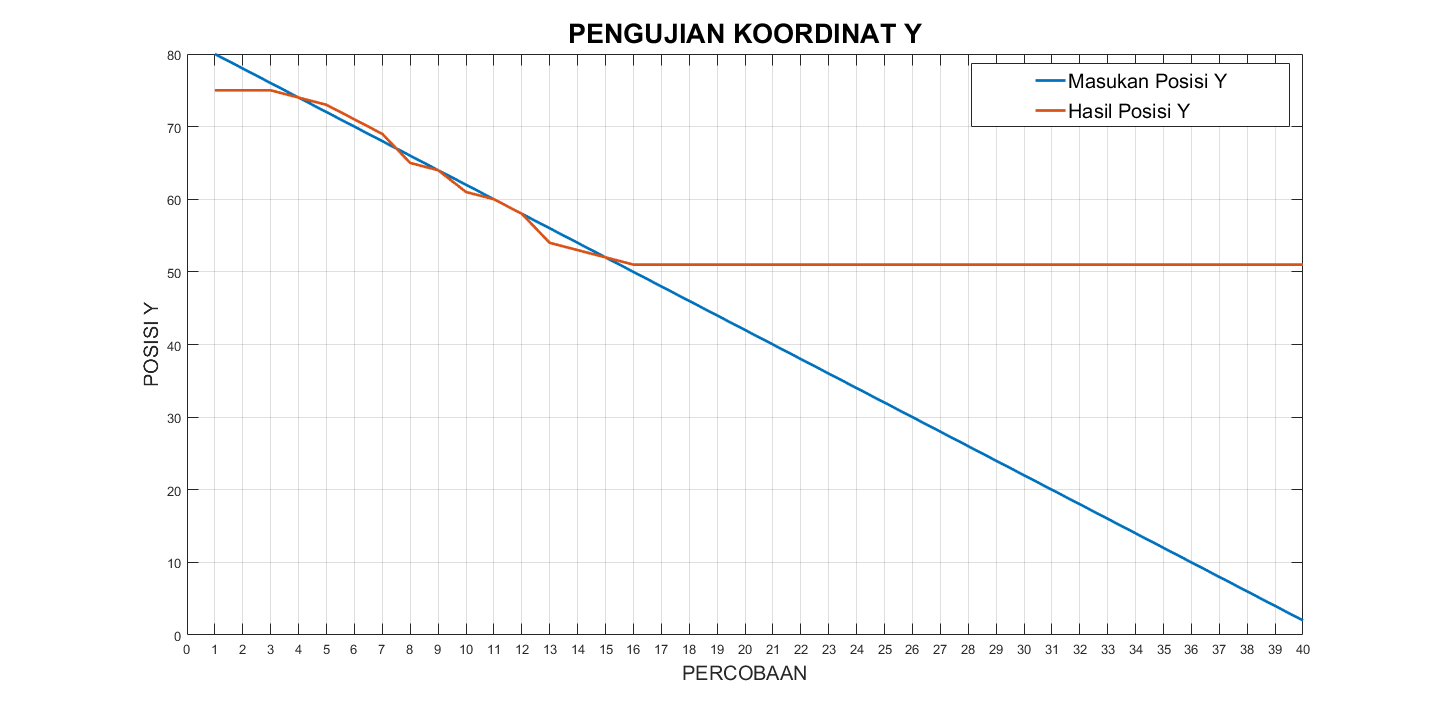
\includegraphics[width=12cm]{gambar/px.png}
	\caption{Grafik Pengujian Koordinat X}
	\label{pic.koordinatx}
\end{figure}

Dari hasil pengujian yang ditampilkan pada Tabel \ref{tbl.x} dan juga Gambar \ref{pic.koordinatx} terlihat bahwa posisi \textit{end-effector} yang dihasilkan pada robot SCARA Serpent dibandingkan dengan data sesuai perhitungan kinematika memiliki sedikit perbedaan pada beberapa data. Perbedaan data ini dapat ditolerasi karena dengan \textit{sampling} koordinat $x$ yang diuji hanya kurang dari lima persen nilai data yang berbeda. Pada hasil yang ditunjukkan diketahui bahwa posisi \textit{end-effector} memiliki batas minimum dan juga maksimum. Batas minimum posisi \textit{end-effector} pada sumbu $x$ yaitu 34 cm dari titik pusat dan batas maksimum posisi \textit{end-effector} pada posisi sumbu $x$ adalah 75 cm yang merupakan panjang dari lengan \textit{shoulder} dan juga lengan \textit{elbow}. Batas ini dapat dilihat bahwa pada Tabel \ref{tbl.x} ketika data masukan diberin nilai kurang dari 34 cm maka posisi \textit{End-Effector} tetap pada posisi 34 cm.


\subsubsection{Pengujian Koordinat Y}

Pengujian koordinat $y$ dilakukan untuk mengetahui batas minimal dan batas maksimal \textit{end-effector} dari \textit{arm manipulator} robot SCARA Serpent relatif terhadap sumbu $y$. Pengujian koordinat $y$ dilakukan dengan cara mengujicobakan setiap titik dari 2 cm sampai dengan total panjang \textit{shoulder} dan \textit{elbow} yaitu 80 cm menggunakan perhitungan kinematika balik. Perhitungan posisi $y$ diujicobakan menggunakan program Processing IDE, sementara untuk pengukuran posisi diukur secara faktual dari posisi \textit{end-effector} dengan membuat sebuah diagram kartesius. Tabel \ref{tbl.y} menunjukkan pengujian koordinat $y$ dan Gambar \ref{pic.koordinaty} menunjukkan grafik dari \textit{sampling} koordinat $y$.
% Please add the following required packages to your document preamble:
% \usepackage{multirow}
% \usepackage[table,xcdraw]{xcolor}
% If you use beamer only pass "xcolor=table" option, i.e. \documentclass[xcolor=table]{beamer}
% \usepackage{longtable}
% Note: It may be necessary to compile the document several times to get a multi-page table to line up properly
\fontsize{8}{10}\selectfont
\begin{longtable}{|c|c|c|c|c|c|}
	\caption{Pengujian Koordinat Y}
	\label{tbl.y}\\
	\hline
	\rowcolor[HTML]{9B9B9B} 
	\cellcolor[HTML]{9B9B9B}                     & \multicolumn{2}{c|}{\cellcolor[HTML]{9B9B9B}X} & \multicolumn{2}{c|}{\cellcolor[HTML]{9B9B9B}Y} & \cellcolor[HTML]{9B9B9B}                           \\ \cline{2-5}
	\rowcolor[HTML]{9B9B9B} 
	\multirow{-2}{*}{\cellcolor[HTML]{9B9B9B}No} & Masukan                & Keluran               & Masukan               & Keluaran               & \multirow{-2}{*}{\cellcolor[HTML]{9B9B9B}Error(\%)} \\ \hline
	\endfirsthead
	%
	\endhead
	%
	1                                            & 0                      & 0                     & 80                    & 75                     & >5                                               \\ \hline
	2                                            & 0                      & 0                     & 78                    & 75                     & 3,84                                       \\ \hline
	3                                            & 0                      & 0                     & 76                    & 75                     & 1,31                                       \\ \hline
	4                                            & 0                      & 0                     & 74                    & 74                     & 0                                                  \\ \hline
	5                                            & 0                      & 0                     & 72                    & 73                     & 1,38                                     \\ \hline
	6                                            & 0                      & 0                     & 70                    & 71                     & 1,42                                       \\ \hline
	7                                            & 0                      & 0                     & 68                    & 69                     & 1,47                                       \\ \hline
	8                                            & 0                      & 0                     & 66                    & 65                     & 1,51                                        \\ \hline
	9                                            & 0                      & 0                     & 64                    & 64                     & 0                                                  \\ \hline
	10                                           & 0                      & 0                     & 62                    & 61                     & 1,6                                        \\ \hline
	11                                           & 0                      & 0                     & 60                    & 60                     & 0                                                  \\ \hline
	12                                           & 0                      & 0                     & 58                    & 58                     & 0                                                  \\ \hline
	13                                           & 0                      & 0                     & 56                    & 54                     & 3,57                                      \\ \hline
	14                                           & 0                      & 0                     & 54                    & 53                     & 1,85                                       \\ \hline
	15                                           & 0                      & 0                     & 52                    & 52                     & 0                                                  \\ \hline
	16                                           & 0                      & 0                     & 50                    & 51                     & 2                                                  \\ \hline
	17                                           & 0                      & 0                     & 48                    & 51                     & >5                                               \\ \hline
	18                                           & 0                      & 0                     & 46                    & 51                     & >5                                        \\ \hline
	19                                           & 0                      & 0                     & 44                    & 51                     & >5                                        \\ \hline
	20                                           & 0                      & 0                     & 42                    & 51                     & >5                                        \\ \hline
	21                                           & 0                      & 0                     & 40                    & 51                     & >5                                               \\ \hline
	22                                           & 0                      & 0                     & 38                    & 51                     & >5                                        \\ \hline
	23                                           & 0                      & 0                     & 36                    & 51                     & >5                                        \\ \hline
	24                                           & 0                      & 0                     & 34                    & 51                     & >5                                                 \\ \hline
	25                                           & 0                      & 0                     & 32                    & 51                     & >5                                            \\ \hline
	26                                           & 0                      & 0                     & 30                    & 51                     & >5                                                 \\ \hline
	27                                           & 0                      & 0                     & 28                    & 51                     & >5                                        \\ \hline
	28                                           & 0                      & 0                     & 26                    & 51                     & >5                                        \\ \hline
	29                                           & 0                      & 0                     & 24                    & 51                     & >5                                              \\ \hline
	30                                           & 0                      & 0                     & 22                    & 51                     & >5                                        \\ \hline
	31                                           & 0                      & 0                     & 20                    & 51                     & >5                                                \\ \hline
	32                                           & 0                      & 0                     & 18                    & 51                     & >5                                        \\ \hline
	33                                           & 0                      & 0                     & 16                    & 51                     & >5                                             \\ \hline
	34                                           & 0                      & 0                     & 14                    & 51                     & >5                                        \\ \hline
	35                                           & 0                      & 0                     & 12                    & 51                     & >5                                                \\ \hline
	36                                           & 0                      & 0                     & 10                    & 51                     & >5                                                \\ \hline
	37                                           & 0                      & 0                     & 8                     & 51                     & >5                                              \\ \hline
	38                                           & 0                      & 0                     & 6                     & 51                     & >5                                                \\ \hline
	39                                           & 0                      & 0                     & 4                     & 51                     & >5                                               \\ \hline
	40                                           & 0                      & 0                     & 2                     & 51                     & >5                                              \\ \hline
\end{longtable}
\fontsize{12}{15}\selectfont
\begin{figure}[H]
	\centering
	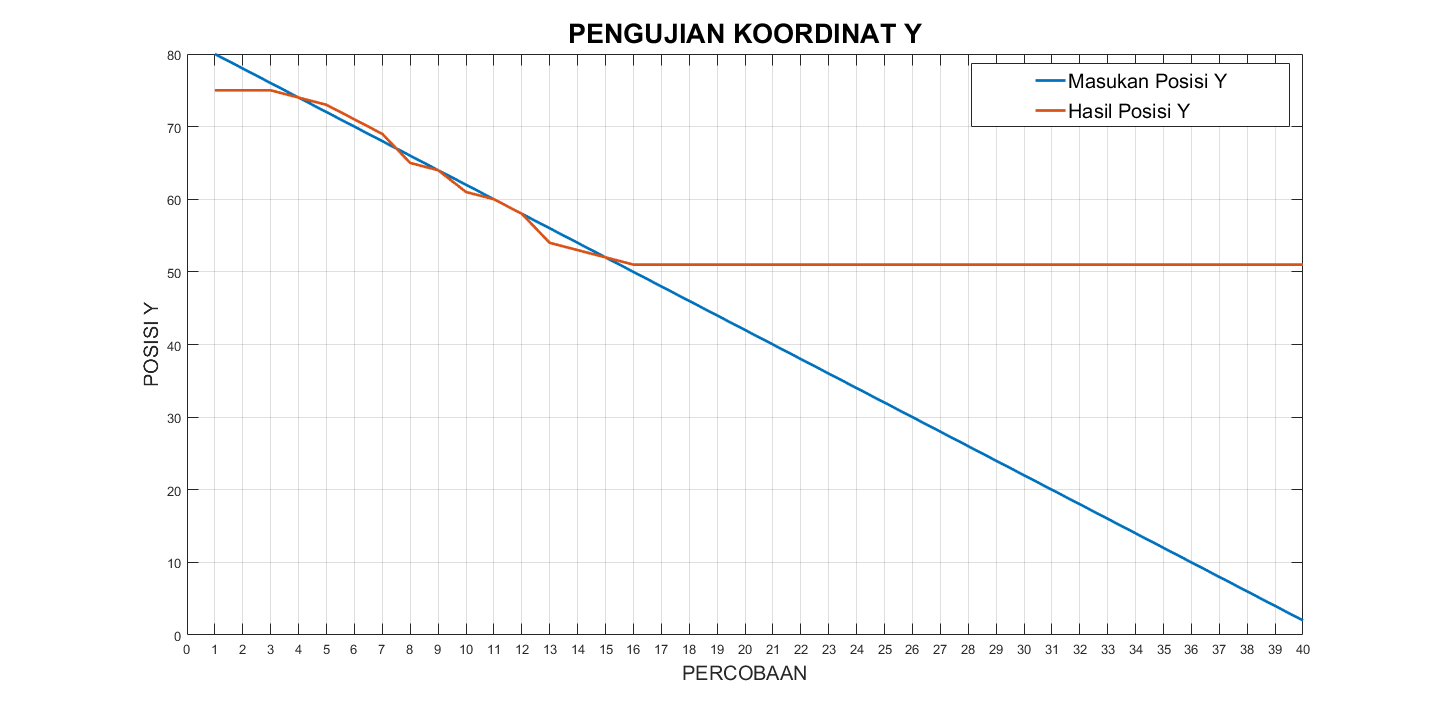
\includegraphics[width=13cm]{gambar/py.png}
	\caption{Grafik Pengujian Koordinat Y}
	\label{pic.koordinaty}
\end{figure}


Dari hasil pengujian yang ditampilkan pada Tabel \ref{tbl.y} dan juga Gambar \ref{pic.koordinaty} terlihat bahwa posisi \textit{end-effector} yang dihasilkan pada robot SCARA Serpent dibandingkan dengan data sesuai perhitungan kinematika memiliki sedikit perbedaan pada beberapa data. Perbedaan data ini dapat ditolerasi karena dengan \textit{sampling} koordinat $y$ yang diuji hanya kurang dari lima persen nilai data yang berbeda. Pada hasil yang ditunjukkan diketahui bahwa posisi \textit{end-effector} memiliki batas minimum dan juga maksimum. Batas minimum posisi \textit{end-effector} pada sumbu $x$ yaitu 51 cm dari titik pusat dan batas maksimum posisi \textit{end-effector} pada posisi sumbu $y$ adalah 75 cm yang merupakan panjang dari lengan \textit{shoulder} dan juga lengan \textit{elbow}.  Batas ini dapat dilihat bahwa pada Tabel \ref{tbl.y} ketika data masukan diberin nilai kurang dari 51 cm maka posisi \textit{end-effector} tetap pada posisi 51 cm.
\subsubsection{\textit{Workspace} Robot Lengan SCARA Serpent }
\textit{Workspace} adalah total volume yang dapat dijangkau oleh \textit{end-effector} robot lengan. Penentuan luas \textit{workspace} ini dibuat dari data pengujian koordinat $x$ dan $y$. Ketinggian maksimum yang dapat dijangkau robot lengan adalah sebesar 25 cm. Jarak minimum yang dapat dijangkau robot lengan pada sumbu $x$ sebesar 31 cm, sementara jarak maksimum yang dapat dijangkau robot lengan sebesar 75 cm. Sedangkan pada sumbu $y$ jarak yang dapat dijangkau robot lengan sebesar 51 cm, sementara jarak maksimum yang dapat dijangkau robot lengan sebesar 75 cm. Titik 0 sampai dengan 31 cm menjadi posisi yang tidak akurat untuk \textit{end-effector} karena jumlah \textit{link} terlalu panjang sedangkan jarak objek terlalu dekat dengan robot lengan, sehingga \textit{end-effector} tidak bisa menjangkau objek pada jarak 0 sampai dengan 31 cm tersebut. Begitupun titik yang lebih dari 75 cm. Jumlah panjang \textit{link} terlalu pendek sedangkan jarak objek terlalu jauh dengan robot lengan, sehingga \textit{end-effector} tidak bida menjangkau objek yang lebih dari 75 cm. Gambar \ref{pic.workpace} merupakan gambaran dari \textit{workspace} yang dihasilkan oleh robot SCARA Serpent.


\begin{figure}[H]
	\centering
	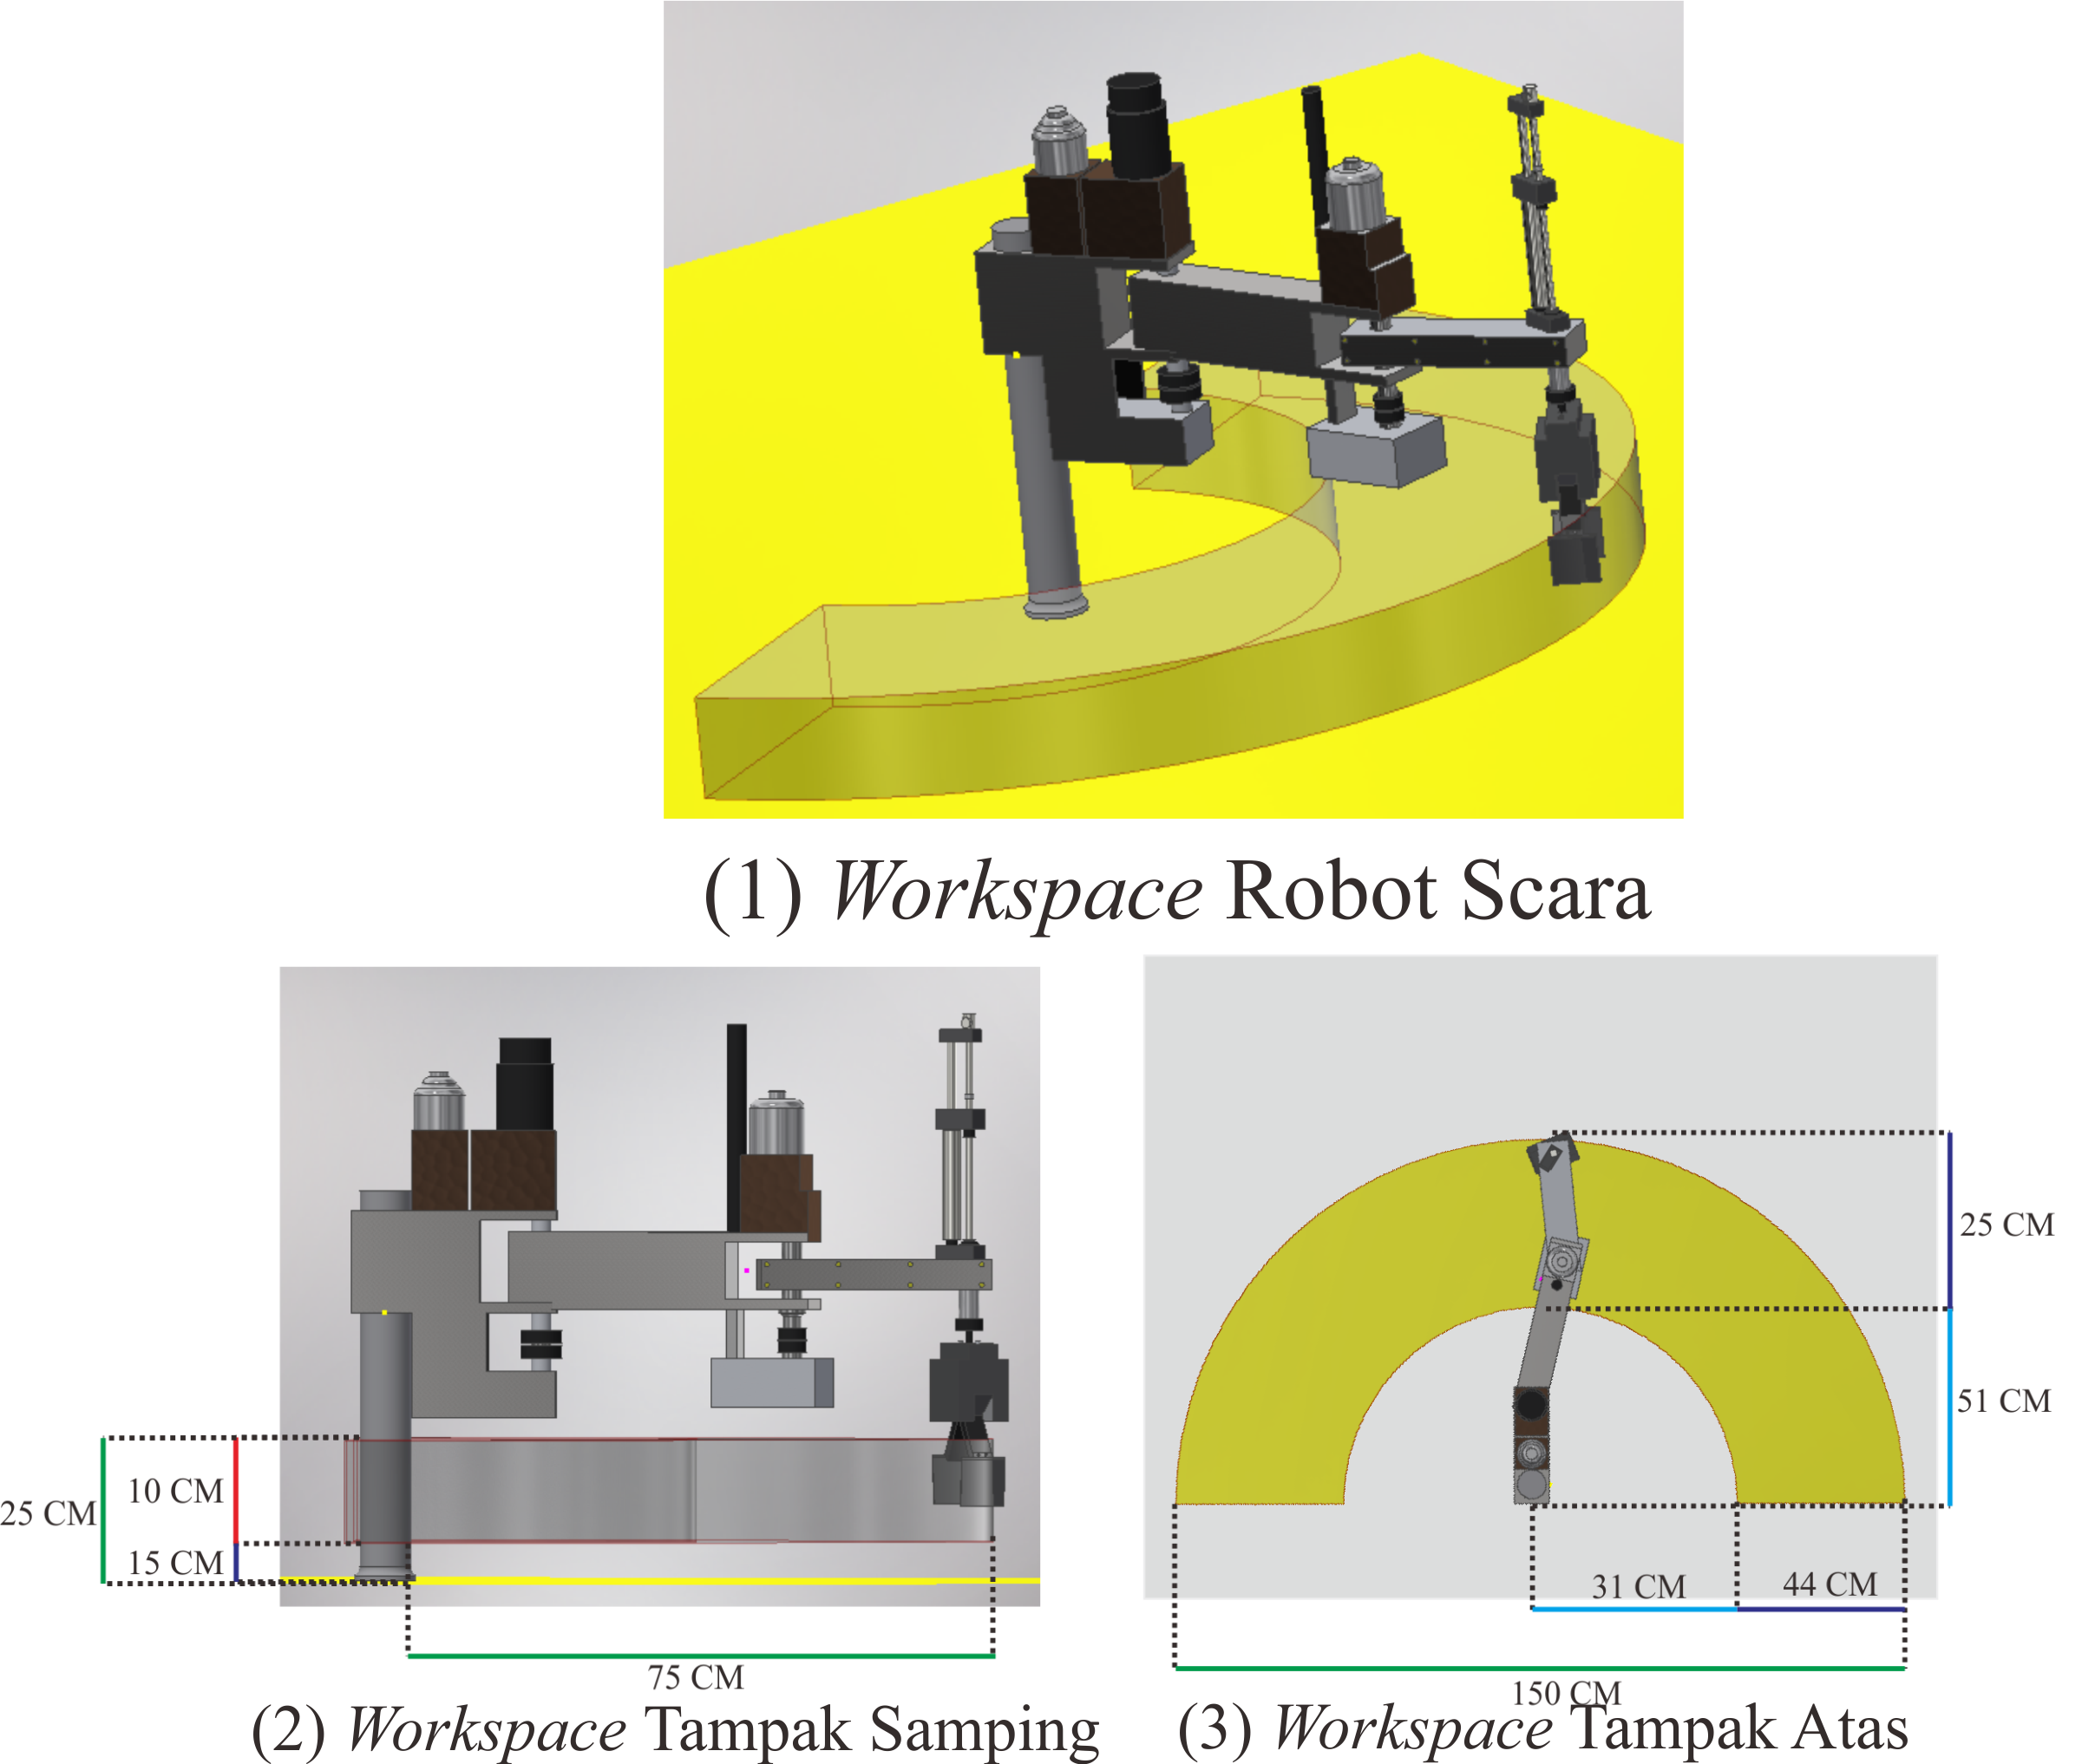
\includegraphics[width=13cm]{gambar/WORKSPACE.png}
	\caption{Workspace Robot SCARA Serpent}
	\label{pic.workpace}
\end{figure}


\subsubsection{Pengujian \textit{Joint Shoulder}}

Pengujian dilakukan dengan cara memberikan sebuah posisi koordinat $x$ dan $y$ dengan nilai yang bervariasi. Nilai tersebut dimasukkan ke dalam sebuah perhitungan kinematika balik yang ada pada program Processing IDE sesuai dengan persamaan pada bab sebelumnya. Hasil yang dihasilkan oleh perhitungan merupakan nilai sudut dari \textit{joint shoulder} dan juga \textit{elbow}. Perhitungan aktual dilakukan dengan cara mengukur sudut pada setiap \textit{joint} menggunakan bantuan busur atau \textit{software} sensor kemiringan yang diunduh pada \textit{smartphone}. Tabel \ref{tbl.shoulder} merupakan hasil pengujian dari \textit{joint shoulder} berdasarkan \textit{sampling} posisi yang diambil. Gambar \ref{pic.jointshoulder} merupakan grafik hubungan dari sudut aktual dan sudut berdasarkan perhitungan kinematika. 
% Please add the following required packages to your document preamble:
% \usepackage[table,xcdraw]{xcolor}
% If you use beamer only pass "xcolor=table" option, i.e. \documentclass[xcolor=table]{beamer}
% \usepackage{longtable}
% Note: It may be necessary to compile the document several times to get a multi-page table to line up properly
\fontsize{8}{10}\selectfont
\begin{longtable}{|c|c|c|c|}
	\caption{Hasil Pengujian \textit{Joint Shoulder}}
	\label{tbl.shoulder}\\
	\hline
	\rowcolor[HTML]{656565} 
	No & Masukan & Keluaran & Error(\%)       \\ \hline
	\endfirsthead
	%
	\endhead
	%
	1  & 0       & 0        & 0           \\ \hline
	2  & 4       & 4        & 0           \\ \hline
	3  & 8       & 8        & 0           \\ \hline
	4  & 12      & 12       & 0           \\ \hline
	5  & 16      & 16       & 0           \\ \hline
	6  & 20      & 20       & 0           \\ \hline
	7  & 24      & 24       & 0           \\ \hline
	8  & 28      & 28       & 0           \\ \hline
	9  & 32      & 33       & 3,12       \\ \hline
	10 & 36      & 35       & 2,77 \\ \hline
	11 & 40      & 40       & 0           \\ \hline
	12 & 44      & 44       & 0           \\ \hline
	13 & 48      & 48       & 0           \\ \hline
	14 & 52      & 52       & 0           \\ \hline
	15 & 56      & 56       & 0           \\ \hline
	16 & 60      & 60       & 0           \\ \hline
	17 & 64      & 64       & 0           \\ \hline
	18 & 68      & 69       & 1,47 \\ \hline
	19 & 72      & 71       & 1,38 \\ \hline
	20 & 76      & 76       & 0           \\ \hline
	21 & 80      & 80       & 0           \\ \hline
	22 & 84      & 84       & 0           \\ \hline
	23 & 88      & 88       & 0           \\ \hline
	24 & 92      & 92       & 0           \\ \hline
	25 & 96      & 96       & 0           \\ \hline
	26 & 100     & 100      & 0           \\ \hline
	27 & 104     & 105      & 0,96 \\ \hline
	28 & 108     & 107      & 0,92 \\ \hline
	29 & 112     & 112      & 0           \\ \hline
	30 & 116     & 116      & 0           \\ \hline
	31 & 120     & 120      & 0           \\ \hline
	32 & 124     & 123      & 0,80 \\ \hline
	33 & 128     & 128      & 0           \\ \hline
	34 & 132     & 132      & 0           \\ \hline
	35 & 136     & 136      & 0           \\ \hline
	36 & 140     & 139      & 0,71 \\ \hline
	37 & 144     & 144      & 0           \\ \hline
	38 & 148     & 148      & 0           \\ \hline
	39 & 152     & 152      & 0           \\ \hline
	40 & 156     & 155      & 0,64 \\ \hline
	41 & 160     & 161      & 0,62       \\ \hline
	42 & 164     & 164      & 0           \\ \hline
	43 & 168     & 168      & 0           \\ \hline
	44 & 172     & 172      & 0           \\ \hline
	45 & 176     & 175      & 0,56 \\ \hline
	46 & 180     & 180      & 0           \\ \hline
\end{longtable}
\fontsize{12}{15}\selectfont
\begin{figure}[H]
	\centering
	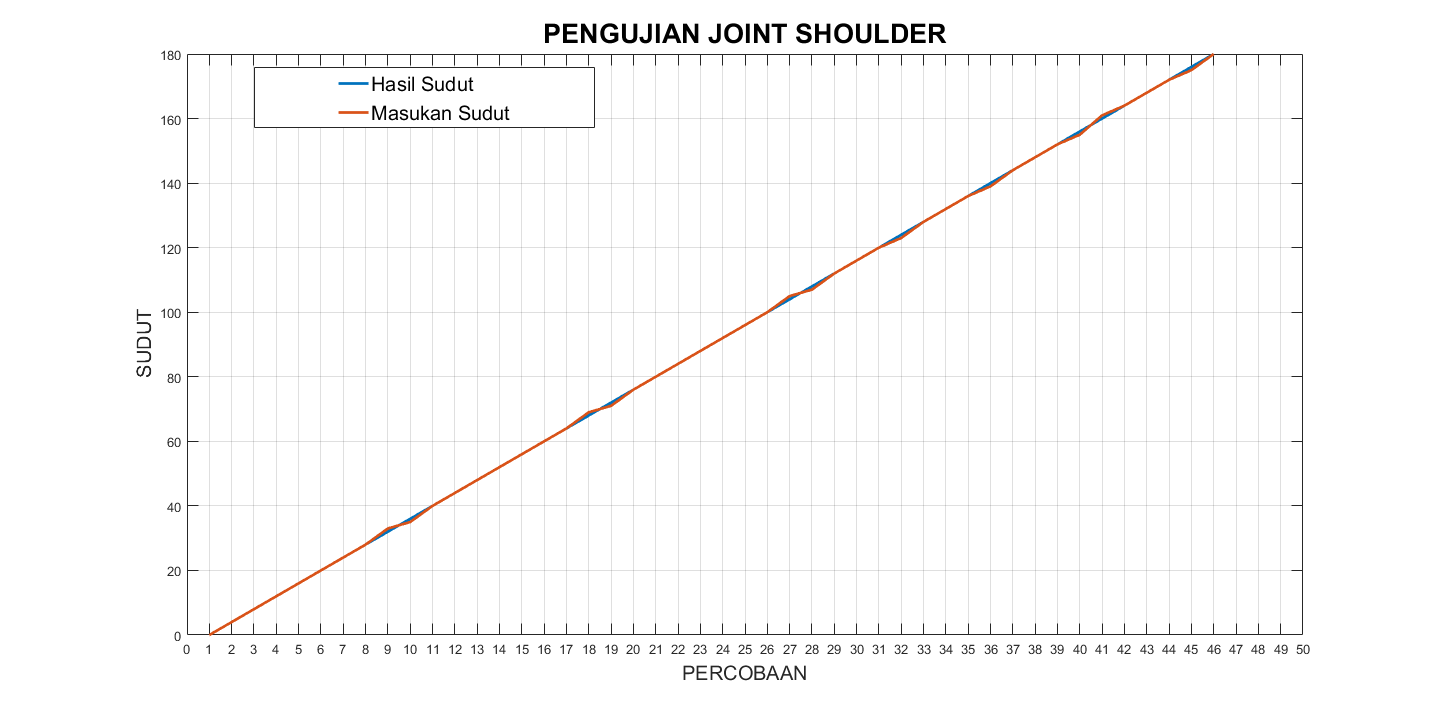
\includegraphics[width=13cm]{gambar/ps.png}
	\caption{Grafik Pengujian \textit{Joint Shoulder}}
	\label{pic.jointshoulder}
\end{figure}

Pada hasil yang ditunjukkan oleh Tabel \ref{tbl.shoulder} dan Gambar \ref{pic.jointshoulder} terlihat bahwa secara keseleuruhan nilai sudut yang dihasilkan oleh aktual pada robot SCARA Serpent dibandingkan dengan perhitungan kinematika oleh Processing IDE tidak begitu terdapat perbedaan. Terlihat bahwa nilai \textit{error}
memiliki nilai minimum 0 persen dan nilai maksimum 2,77 persen. Persentase \textit{error} didapat dari data yang tidak sesuai dibagi oleh keleluruhan data yang diuji coba. Dapat dikatakan bahwa pengujian sudut \textit{joint shoulder} cukup baik.

\subsubsection{Pengujian \textit{Joint Elbow}}

Pengujian \textit{joint elbow} dilakukan dengan membandingkan nilai sudut yang dihasilkan oleh perhitungan kinematika yang ada pada program Processing IDE dengan sudut yang dihasilkan dalam aktual robot SCARA Serpent. Pengujian dilakukan dengan cara memberikan sebuah posisi koordinat $x$ dan $y$ dengan nilai yang bervariasi. Nilai tersebut dimasukkan ke dalam sebuah perhitungan kinematika balik yang ada pada program Processing IDE. Hasil yang dihasilkan oleh perhitungan merupakan nilai sudut dari \textit{joint shoulder} dan juga \textit{elbow}. Perhitungan aktual dilakukan dengan cara mengukur sudut pada setiap \textit{joint} menggunakan bantuan busur atau \textit{software} sensor kemiringan yang diunduh pada \textit{smartphone}. Tabel \ref{tbl.elbow} merupakan hasil pengujian dari \textit{joint elbow} berdasarkan \textit{sampling} posisi yang diambil. Gambar \ref{pic.jointelbow} merupakan grafik hubungan dari sudut aktual dan sudut berdasarkan perhitungan kinematika. 
% Please add the following required packages to your document preamble:
% \usepackage[table,xcdraw]{xcolor}
% If you use beamer only pass "xcolor=table" option, i.e. \documentclass[xcolor=table]{beamer}
% \usepackage{longtable}
% Note: It may be necessary to compile the document several times to get a multi-page table to line up properly
\fontsize{8}{10}\selectfont
\begin{longtable}{|c|c|c|c|}
	\caption{Hasil Pengujian \textit{Joint Elbow}}
	\label{tbl.elbow}\\
	\hline
	\rowcolor[HTML]{656565} 
	No & Masukan & Keluaran & Error(\%)       \\ \hline
	\endfirsthead
	%
	\endhead
	%
	1  & 0       & 1        & 0           \\ \hline
	2  & 4       & 4        & 0           \\ \hline
	3  & 8       & 9        & >5      \\ \hline
	4  & 12      & 13       & >5  \\ \hline
	5  & 16      & 17       & >5         \\ \hline
	6  & 20      & 21       & 5           \\ \hline
	7  & 24      & 25       & 4,16 \\ \hline
	8  & 28      & 29       & 3,57 \\ \hline
	9  & 32      & 32       & 0           \\ \hline
	10 & 36      & 36       & 0           \\ \hline
	11 & 40      & 41       & 2,5         \\ \hline
	12 & 44      & 45       & 2,27 \\ \hline
	13 & 48      & 49       & 2,08 \\ \hline
	14 & 52      & 53       & 1,92 \\ \hline
	15 & 56      & 57       & 1,78 \\ \hline
	16 & 60      & 61       & 1,66 \\ \hline
	17 & 64      & 64       & 0           \\ \hline
	18 & 68      & 67       & 1,47 \\ \hline
	19 & 72      & 72       & 0           \\ \hline
	20 & 76      & 76       & 0           \\ \hline
	21 & 80      & 80       & 0           \\ \hline
	22 & 84      & 84       & 0           \\ \hline
	23 & 88      & 88       & 0           \\ \hline
	24 & 92      & 92       & 0           \\ \hline
	25 & 96      & 96       & 0           \\ \hline
	26 & 100     & 100      & 0           \\ \hline
	27 & 104     & 104      & 0           \\ \hline
	28 & 108     & 108      & 0           \\ \hline
	29 & 112     & 111      & 0,89 \\ \hline
	30 & 116     & 115      & 0,86 \\ \hline
	31 & 120     & 119      & 0,83 \\ \hline
	32 & 124     & 123      & 0,80 \\ \hline
	33 & 128     & 128      & 0           \\ \hline
	34 & 132     & 132      & 0           \\ \hline
	35 & 136     & 136      & 0           \\ \hline
	36 & 140     & 140      & 0           \\ \hline
	37 & 144     & 144      & 0           \\ \hline
	38 & 148     & 148      & 0           \\ \hline
	39 & 152     & 152      & 0           \\ \hline
	40 & 156     & 156      & 0           \\ \hline
	41 & 160     & 160      & 0           \\ \hline
	42 & 164     & 164      & 0           \\ \hline
	43 & 168     & 168      & 0           \\ \hline
	44 & 172     & 172      & 0           \\ \hline
	45 & 176     & 176      & 0           \\ \hline
	46 & 180     & 180      & 0           \\ \hline
\end{longtable}
\fontsize{12}{15}\selectfont
\begin{figure}[H]
	\centering
	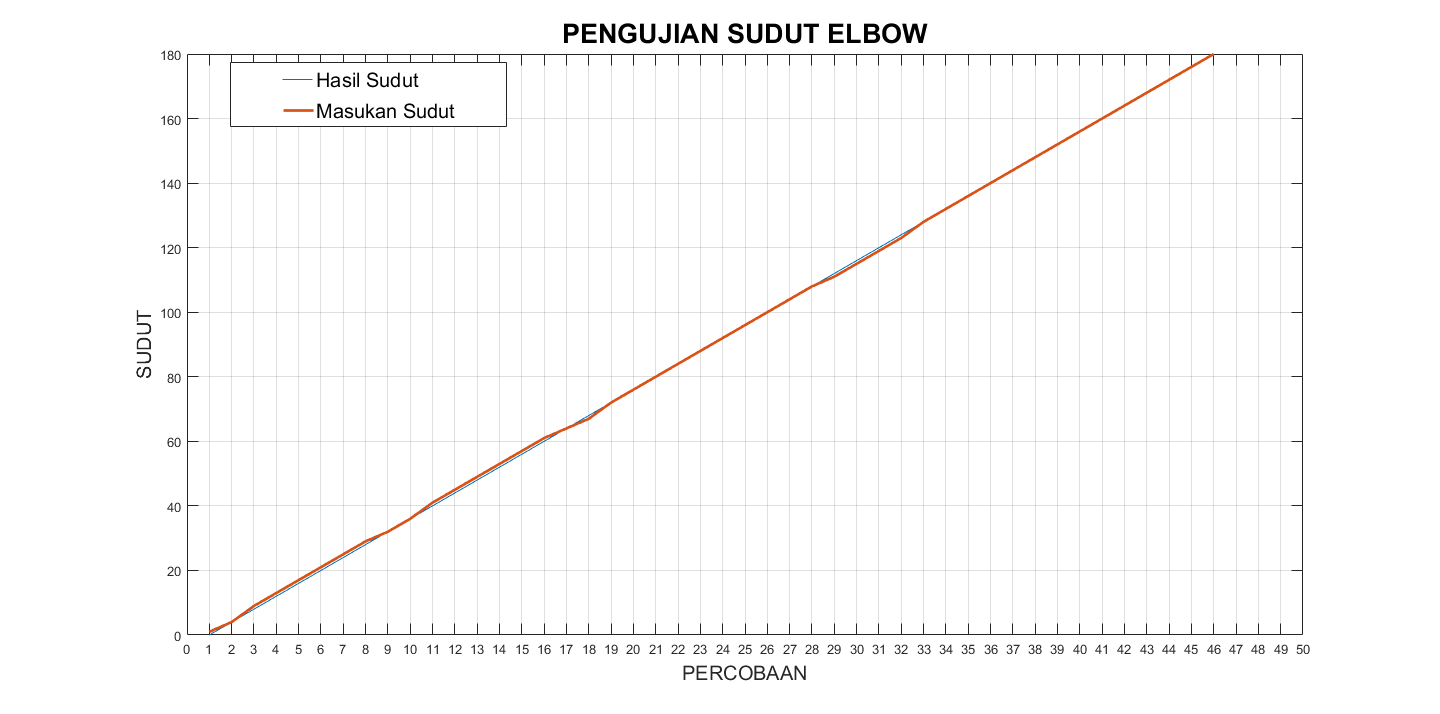
\includegraphics[width=12cm]{gambar/pe.png}
	\caption{Grafik Pengujian \textit{Joint Elbow}}
	\label{pic.jointelbow}
\end{figure}

Pada hasil yang ditunjukkan oleh Tabel \ref{tbl.elbow} dan Gambar \ref{pic.jointelbow} terlihat bahwa secara keseleuruhan nilai sudut yang dihasilkan oleh aktual pada robot SCARA Serpent dibandingkan dengan perhitungan kinematika oleh Processing IDE tidak begitu terdapat perbedaan. Terlihat bahwa nilai \textit{error}
memiliki nilai minimum 0 persen dan nilai maksimum lebih dari 5 persen. Persentase \textit{error} didapat dari data yang tidak sesuai dibagi oleh keleluruhan data yang diuji coba. 


\section{Pengujian Keseluruhan}
Setelah semua komponen sistem yang diuji dapat bekerja dengan baik, pengujian selanjutnya adalah pengujian sistem secara keseluruhan dengan beberapa parameter uji yang diberikan. Parameter uji tersebut diantaranya adalah pengujian akurasi robot lengan, dan simulasi robot lengan. 

\subsection{Pengujian Akurasi Robot Lengan}

Pada pengujian akurasi robot lengan dilakukan pengujian dengan memberikan posisi koordinat $x$ dan $y$ dan melihat kembali posisi $x$ dan $y$ secara aktual, melihat besar sudut pada masing-masing \textit{joint} dengan perbandingan perhitungan kinematika. Pengujian akurasi robot lengan ini akan menghasilkan sebuah hasil secara luas dan dapat ditarik untuk sebuah kesimpulan yang menentukan robot SCARA Serpent dapat bekerja baik atau buruk secara keseluruhan. Tabel \ref{tbl.akurasikeseluruhan} merupakan hasil dari pengujian akurasi robot lengan secara keseluruhan. Gambar \ref{pic.akurasikeseluruhan} merupakan grafik dari hasil pengujian akurasi robot lengan secara keseluruhan.
% Please add the following required packages to your document preamble:
% \usepackage{multirow}
% \usepackage{graphicx}
% \usepackage[table,xcdraw]{xcolor}
% If you use beamer only pass "xcolor=table" option, i.e. \documentclass[xcolor=table]{beamer}
\begin{table}[H]
	\caption{}
	\label{tbl.akurasikeseluruhan}
	\resizebox{\textwidth}{!}{%
		\begin{tabular}{|
				>{\columncolor[HTML]{FFCCC9}}c |
				>{\columncolor[HTML]{FFCCC9}}c |
				>{\columncolor[HTML]{FFCCC9}}c |
				>{\columncolor[HTML]{FFCCC9}}c |
				>{\columncolor[HTML]{FFCCC9}}c |
				>{\columncolor[HTML]{FFFC9E}}c |
				>{\columncolor[HTML]{FFFC9E}}c |
				>{\columncolor[HTML]{FFFC9E}}c |
				>{\columncolor[HTML]{FFCCC9}}c |
				>{\columncolor[HTML]{FFCCC9}}c |
				>{\columncolor[HTML]{FFCCC9}}c |
				>{\columncolor[HTML]{FFFC9E}}c |}
			\hline
			\multicolumn{5}{|c|}{\cellcolor[HTML]{9B9B9B}Posisi (x,y)} & \multicolumn{3}{c|}{\cellcolor[HTML]{9B9B9B}Shoulder} & \multicolumn{3}{c|}{\cellcolor[HTML]{9B9B9B}Elbow} & \cellcolor[HTML]{9B9B9B} \\ \cline{1-11}
			\multicolumn{2}{|c|}{\cellcolor[HTML]{9B9B9B}Input} & \multicolumn{2}{c|}{\cellcolor[HTML]{9B9B9B}Output} & \cellcolor[HTML]{9B9B9B} & \cellcolor[HTML]{9B9B9B} & \cellcolor[HTML]{9B9B9B} & \cellcolor[HTML]{9B9B9B} & \cellcolor[HTML]{9B9B9B} & \cellcolor[HTML]{9B9B9B} & \cellcolor[HTML]{9B9B9B} & \cellcolor[HTML]{9B9B9B} \\ \cline{1-4}
			\cellcolor[HTML]{9B9B9B}x & \cellcolor[HTML]{9B9B9B}y & \cellcolor[HTML]{9B9B9B}x & \cellcolor[HTML]{9B9B9B}y & \multirow{-2}{*}{\cellcolor[HTML]{9B9B9B}Error(\%)} & \multirow{-2}{*}{\cellcolor[HTML]{9B9B9B}Hasil} & \multirow{-2}{*}{\cellcolor[HTML]{9B9B9B}Terukur} & \multirow{-2}{*}{\cellcolor[HTML]{9B9B9B}Error(\%)} & \multirow{-2}{*}{\cellcolor[HTML]{9B9B9B}Hasil} & \multirow{-2}{*}{\cellcolor[HTML]{9B9B9B}Terukur} & \multirow{-2}{*}{\cellcolor[HTML]{9B9B9B}Error(\%)} & \multirow{-3}{*}{\cellcolor[HTML]{9B9B9B}Error Total(\%)} \\ \hline
			0 & 76 & 0 & 75 & Error & 90 & 90,0 & 0,00 & 0 & 0 & Error & Error \\ \hline
			2 & 74 & 2 & 74 & 0,00 & 96 & 95,0 & 0,73 & 16,59 & 16 & 3,56 & 1,43 \\ \hline
			4 & 72 & 4 & 72 & 0,00 & 98,82 & 99,0 & 0,18 & 27,79 & 26 & 6,44 & 2,21 \\ \hline
			6 & 70 & 4 & 70 & 16,67 & 102,66 & 102,0 & 0,64 & 39,5 & 40 & 1,27 & 6,19 \\ \hline
			8 & 68 & 6 & 67 & 13,24 & 104,31 & 103,0 & 1,26 & 48,04 & 48 & 0,08 & 4,86 \\ \hline
			10 & 66 & 9 & 66 & 5,00 & 104,18 & 103,0 & 1,13 & 52,36 & 52 & 0,69 & 2,27 \\ \hline
			12 & 64 & 10 & 64 & 8,33 & 105,2 & 104,0 & 1,14 & 58,63 & 58 & 1,07 & 3,52 \\ \hline
			14 & 62 & 12 & 62 & 7,14 & 105,22 & 104,0 & 1,16 & 64,13 & 64 & 0,20 & 2,84 \\ \hline
			16 & 60 & 14 & 60 & 6,25 & 103,95 & 104,0 & 0,05 & 66,68 & 66 & 1,02 & 2,44 \\ \hline
			18 & 58 & 15 & 59 & 7,47 & 104,08 & 103,0 & 1,04 & 71,58 & 71 & 0,81 & 3,11 \\ \hline
			20 & 56 & 18 & 58 & 3,21 & 102,32 & 102,0 & 0,31 & 73,39 & 73 & 0,53 & 1,35 \\ \hline
			22 & 54 & 20 & 55 & 3,62 & 101,01 & 100,0 & 1,00 & 76,85 & 76 & 1,11 & 1,91 \\ \hline
			24 & 52 & 21 & 54 & 4,33 & 100,03 & 100,0 & 0,03 & 80,18 & 81 & 1,02 & 1,79 \\ \hline
			26 & 50 & 24 & 52 & 1,85 & 97,83 & 97,0 & 0,85 & 81,33 & 81 & 0,41 & 1,03 \\ \hline
			28 & 48 & 26 & 50 & 1,49 & 95,48 & 95,0 & 0,50 & 83,2 & 82 & 1,44 & 1,14 \\ \hline
			30 & 46 & 28 & 48 & 1,16 & 94,01 & 94,0 & 0,01 & 85,9 & 83 & 3,38 & 1,52 \\ \hline
			32 & 44 & 30 & 47 & 0,28 & 91,07 & 92,0 & 1,02 & 85,71 & 84 & 2,00 & 1,10 \\ \hline
			34 & 42 & 32 & 44 & 0,56 & 88,07 & 89,0 & 1,06 & 86,65 & 86 & 0,75 & 0,79 \\ \hline
			36 & 40 & 34 & 43 & 0,97 & 86,01 & 87,0 & 1,15 & 87,02 & 87 & 0,02 & 0,72 \\ \hline
			38 & 38 & 36 & 42 & 2,63 & 82,83 & 84,0 & 1,41 & 87,41 & 87 & 0,47 & 1,50 \\ \hline
			40 & 36 & 39 & 40 & 4,31 & 79,33 & 80,0 & 0,84 & 87,02 & 87 & 0,02 & 1,72 \\ \hline
			42 & 34 & 40 & 36 & 0,56 & 76,78 & 76,0 & 1,02 & 87,8 & 87 & 0,91 & 0,83 \\ \hline
			44 & 32 & 43 & 36 & 5,11 & 73,23 & 73,0 & 0,31 & 85,71 & 86 & 0,34 & 1,92 \\ \hline
			46 & 30 & 44 & 34 & 4,49 & 70,45 & 72,0 & 2,20 & 85,9 & 86 & 0,12 & 2,27 \\ \hline
			48 & 28 & 47 & 33 & 7,89 & 66,8 & 66,0 & 1,20 & 83,2 & 84 & 0,96 & 3,35 \\ \hline
			50 & 26 & 49 & 31 & 8,62 & 62,92 & 62,0 & 1,46 & 81,33 & 83 & 2,05 & 4,04 \\ \hline
			52 & 24 & 52 & 28 & 8,33 & 58,87 & 58,0 & 1,48 & 78,65 & 78 & 0,83 & 3,55 \\ \hline
			54 & 22 & 53 & 26 & 8,16 & 56,09 & 55,0 & 1,94 & 76,85 & 77 & 0,20 & 3,43 \\ \hline
			56 & 20 & 56 & 25 & 12,50 & 51,9 & 51,0 & 1,73 & 73,39 & 75 & 2,19 & 5,48 \\ \hline
			58 & 18 & 58 & 23 & 13,89 & 49,07 & 49,0 & 0,14 & 70,93 & 71 & 0,10 & 4,71 \\ \hline
			60 & 16 & 60 & 21 & 15,63 & 44,62 & 44,0 & 1,39 & 66,68 & 65 & 2,52 & 6,51 \\ \hline
			62 & 14 & 62 & 18 & 14,29 & 40,2 & 40,0 & 0,50 & 62,12 & 64 & 3,03 & 5,94 \\ \hline
			64 & 12 & 64 & 16 & 16,67 & 36,92 & 37,0 & 0,22 & 58,21 & 58 & 0,36 & 5,75 \\ \hline
			66 & 10 & 66 & 14 & 20,00 & 32,11 & 33,0 & 2,77 & 52,36 & 53 & 1,22 & 8,00 \\ \hline
			68 & 8 & 68 & 12 & 25,00 & 28,23 & 29,0 & 2,73 & 48,04 & 48 & 0,08 & 9,27 \\ \hline
			70 & 6 & 70 & 10 & 33,33 & 22,91 & 24,0 & 4,76 & 39,17 & 40 & 2,12 & 13,40 \\ \hline
			72 & 4 & 73 & 8 & 50,69 & 15,91 & 18,0 & 13,14 & 27,79 & 28 & 0,76 & 21,53 \\ \hline
			74 & 2 & 74 & 5 & 75,00 & 9,08 & 12,0 & 32,16 & 16,59 & 17 & 2,47 & 36,54 \\ \hline
			76 & 0 & 75 & 2 & Error & 0 & 2,0 & Error & 0 & 2 & Error & Error \\ \hline
			\multicolumn{4}{|c|}{\cellcolor[HTML]{FFCCC9}TOTAL} & 408,67 & \multicolumn{2}{c|}{\cellcolor[HTML]{FFFC9E}TOTAL} & 84,67 & \multicolumn{2}{c|}{\cellcolor[HTML]{FFCCC9}TOTAL} & 46,54 & 179,96 \\ \hline
			\multicolumn{4}{|c|}{\cellcolor[HTML]{FFCCC9}RATA-RATA} & 10,48 & \multicolumn{2}{c|}{\cellcolor[HTML]{FFFC9E}RATA-RATA} & 2,17 & \multicolumn{2}{c|}{\cellcolor[HTML]{FFCCC9}RATA-RATA} & 1,19 & 4,61 \\ \hline
		\end{tabular}%
	}
\end{table}

\fontsize{12}{15}\selectfont
\begin{table}[H]
	\centering
	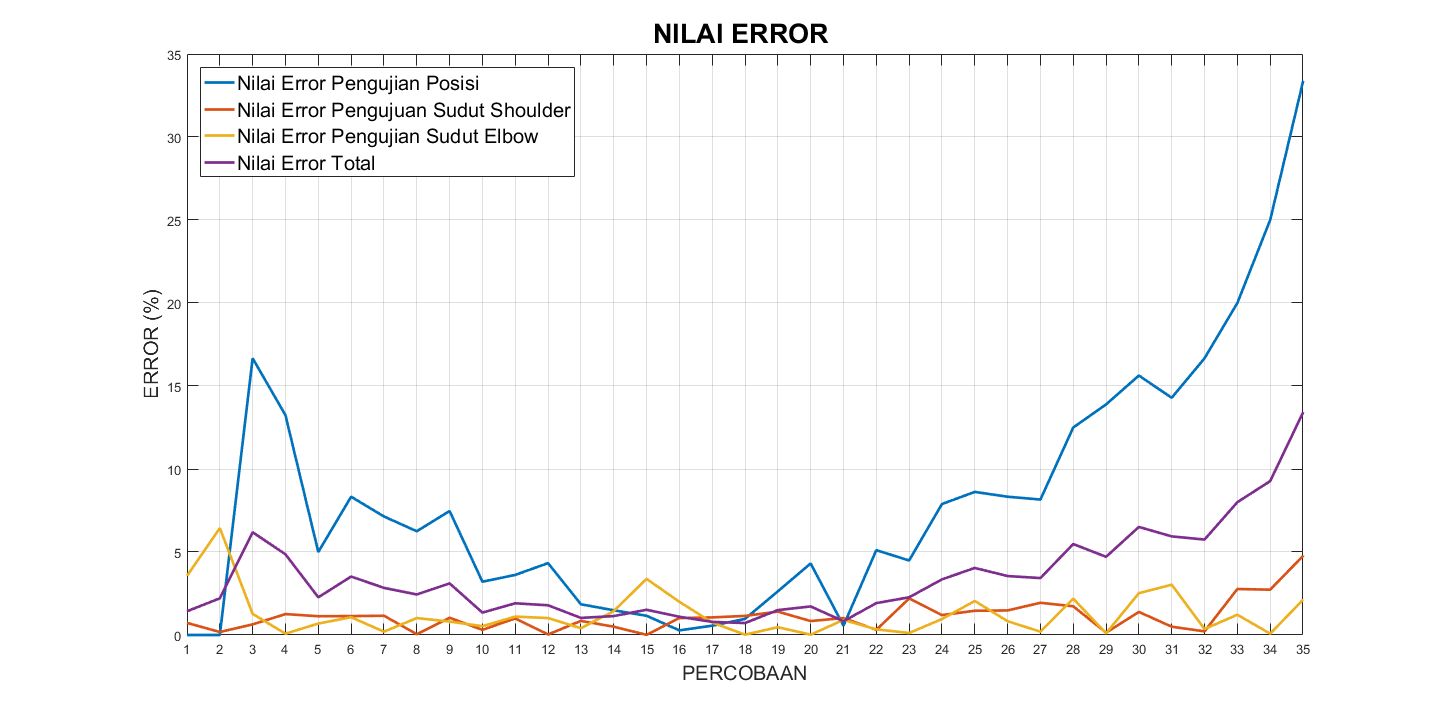
\includegraphics[width=13cm]{gambar/ne.png}
	\caption{Grafik Pengujian Akurasi Robot Secara Keseluruhan}
	\label{pic.akurasikeseluruhan}
\end{table}


Pada hasil pengujian yang ditunjukkan pada Tabel \ref{tbl.akurasikeseluruhan} dan Gambar \ref{pic.akurasikeseluruhan} terlihat bahwa pengujian mendapat beberapa data yang beragam. Terlihat bahwa nilai kesalahan paling banyak terdapat pada bagian posisi koordinat $x$ dan $y$ dan kesalahan paling sedikit pada bagian sudut \textit{shoulder}. Sedangkan untuk sistem keseluruhan kesalahan total pada akurasi robot memiliki nilai 4,61 persen. Nilai sebesar ini merupakan nilai yang cukup baik bagi sebuah sistem. Dengan nilai tersebut maka sistem kinematika robot SCARA Serpent ini dapat dikatakan baik. 


\section{Pengujian Kendali Proposional}
Tujuan dari kendali proposional pada sistem ini adalah membuat robot mampu menuju sebuah sudut yang diinginkan dengan tingkat \textit{error} paling minimum. Sudut pada robot lengan ini merupakan sudut yang terletak pada \textit{joint shoulder, elbow} dan \textit{end-effector}. Semakin kecil nilai \textit{error} yang dihasilkan dari pengujian ini maka semakin baik pergerakan dari robot lengan. Gambar \ref{pic.kendali} merupakan data pengujian dari robot lengan dengan variasi nilai kendali proposional yang menghasilkan respon yang berbeda-beda.


\begin{figure}[H]
	\centering
	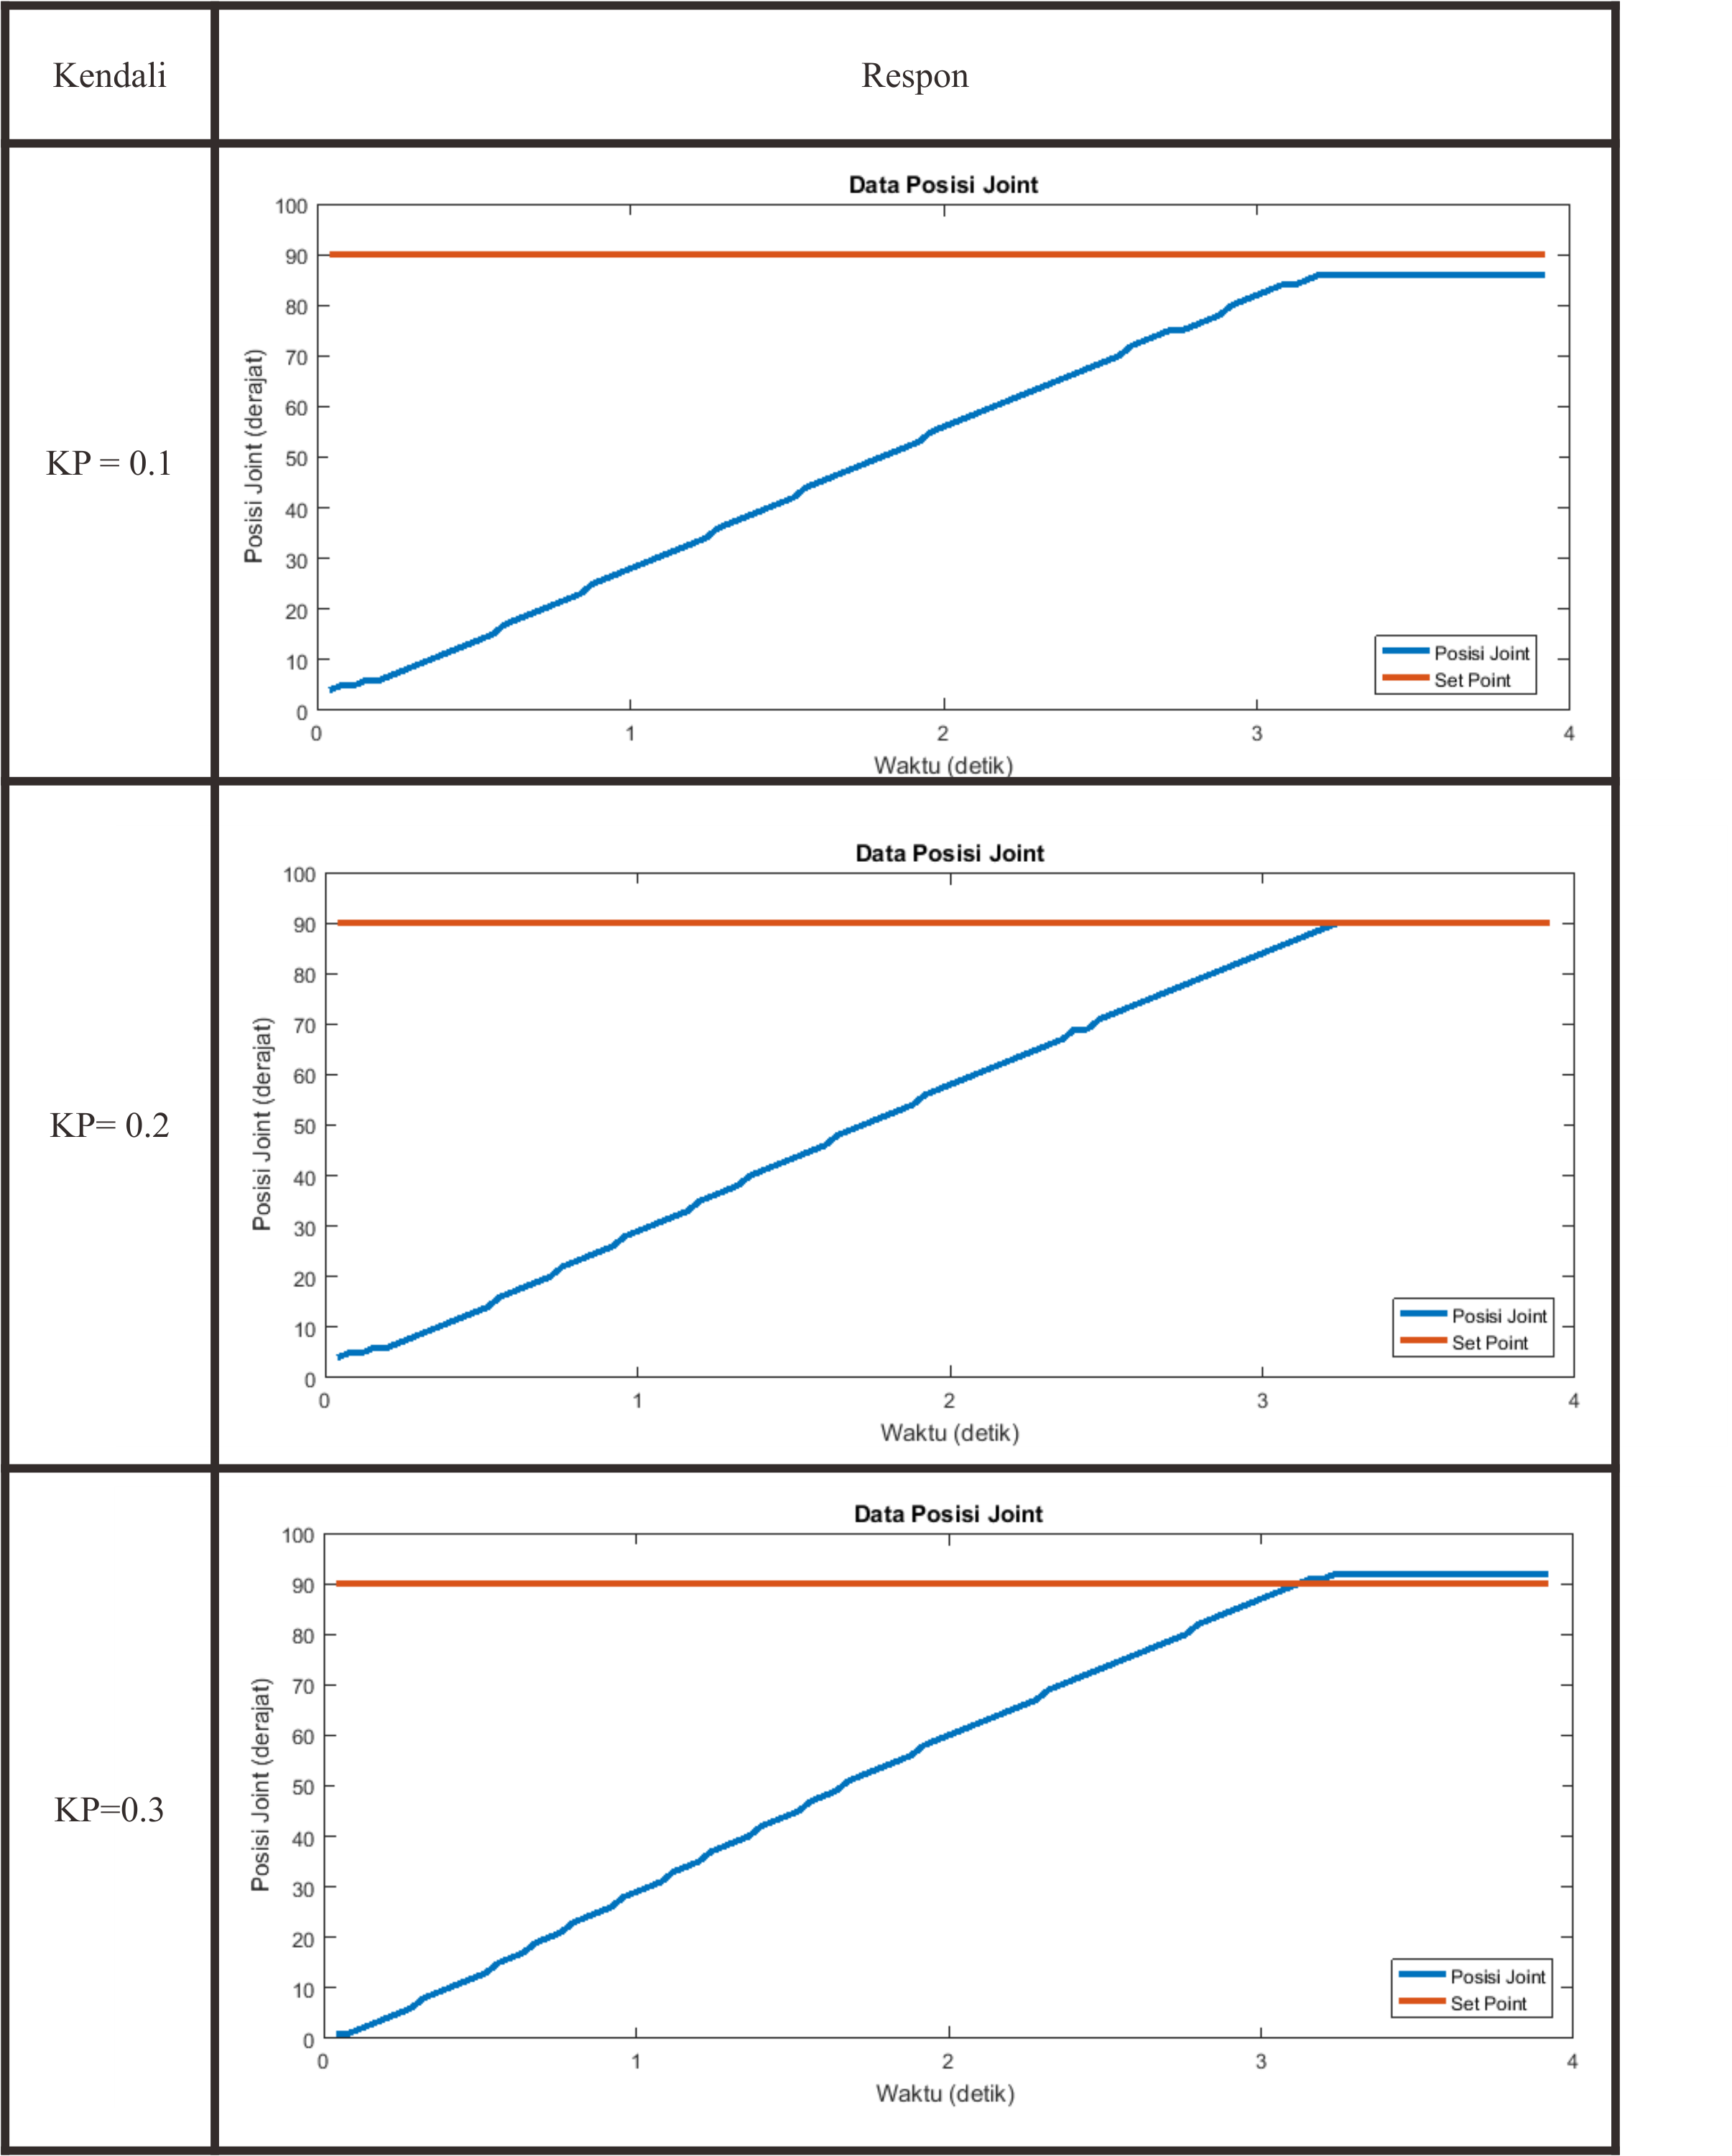
\includegraphics[width=13cm]{gambar/kendali1.png}
\end{figure}

\begin{figure}[H]
	\centering
	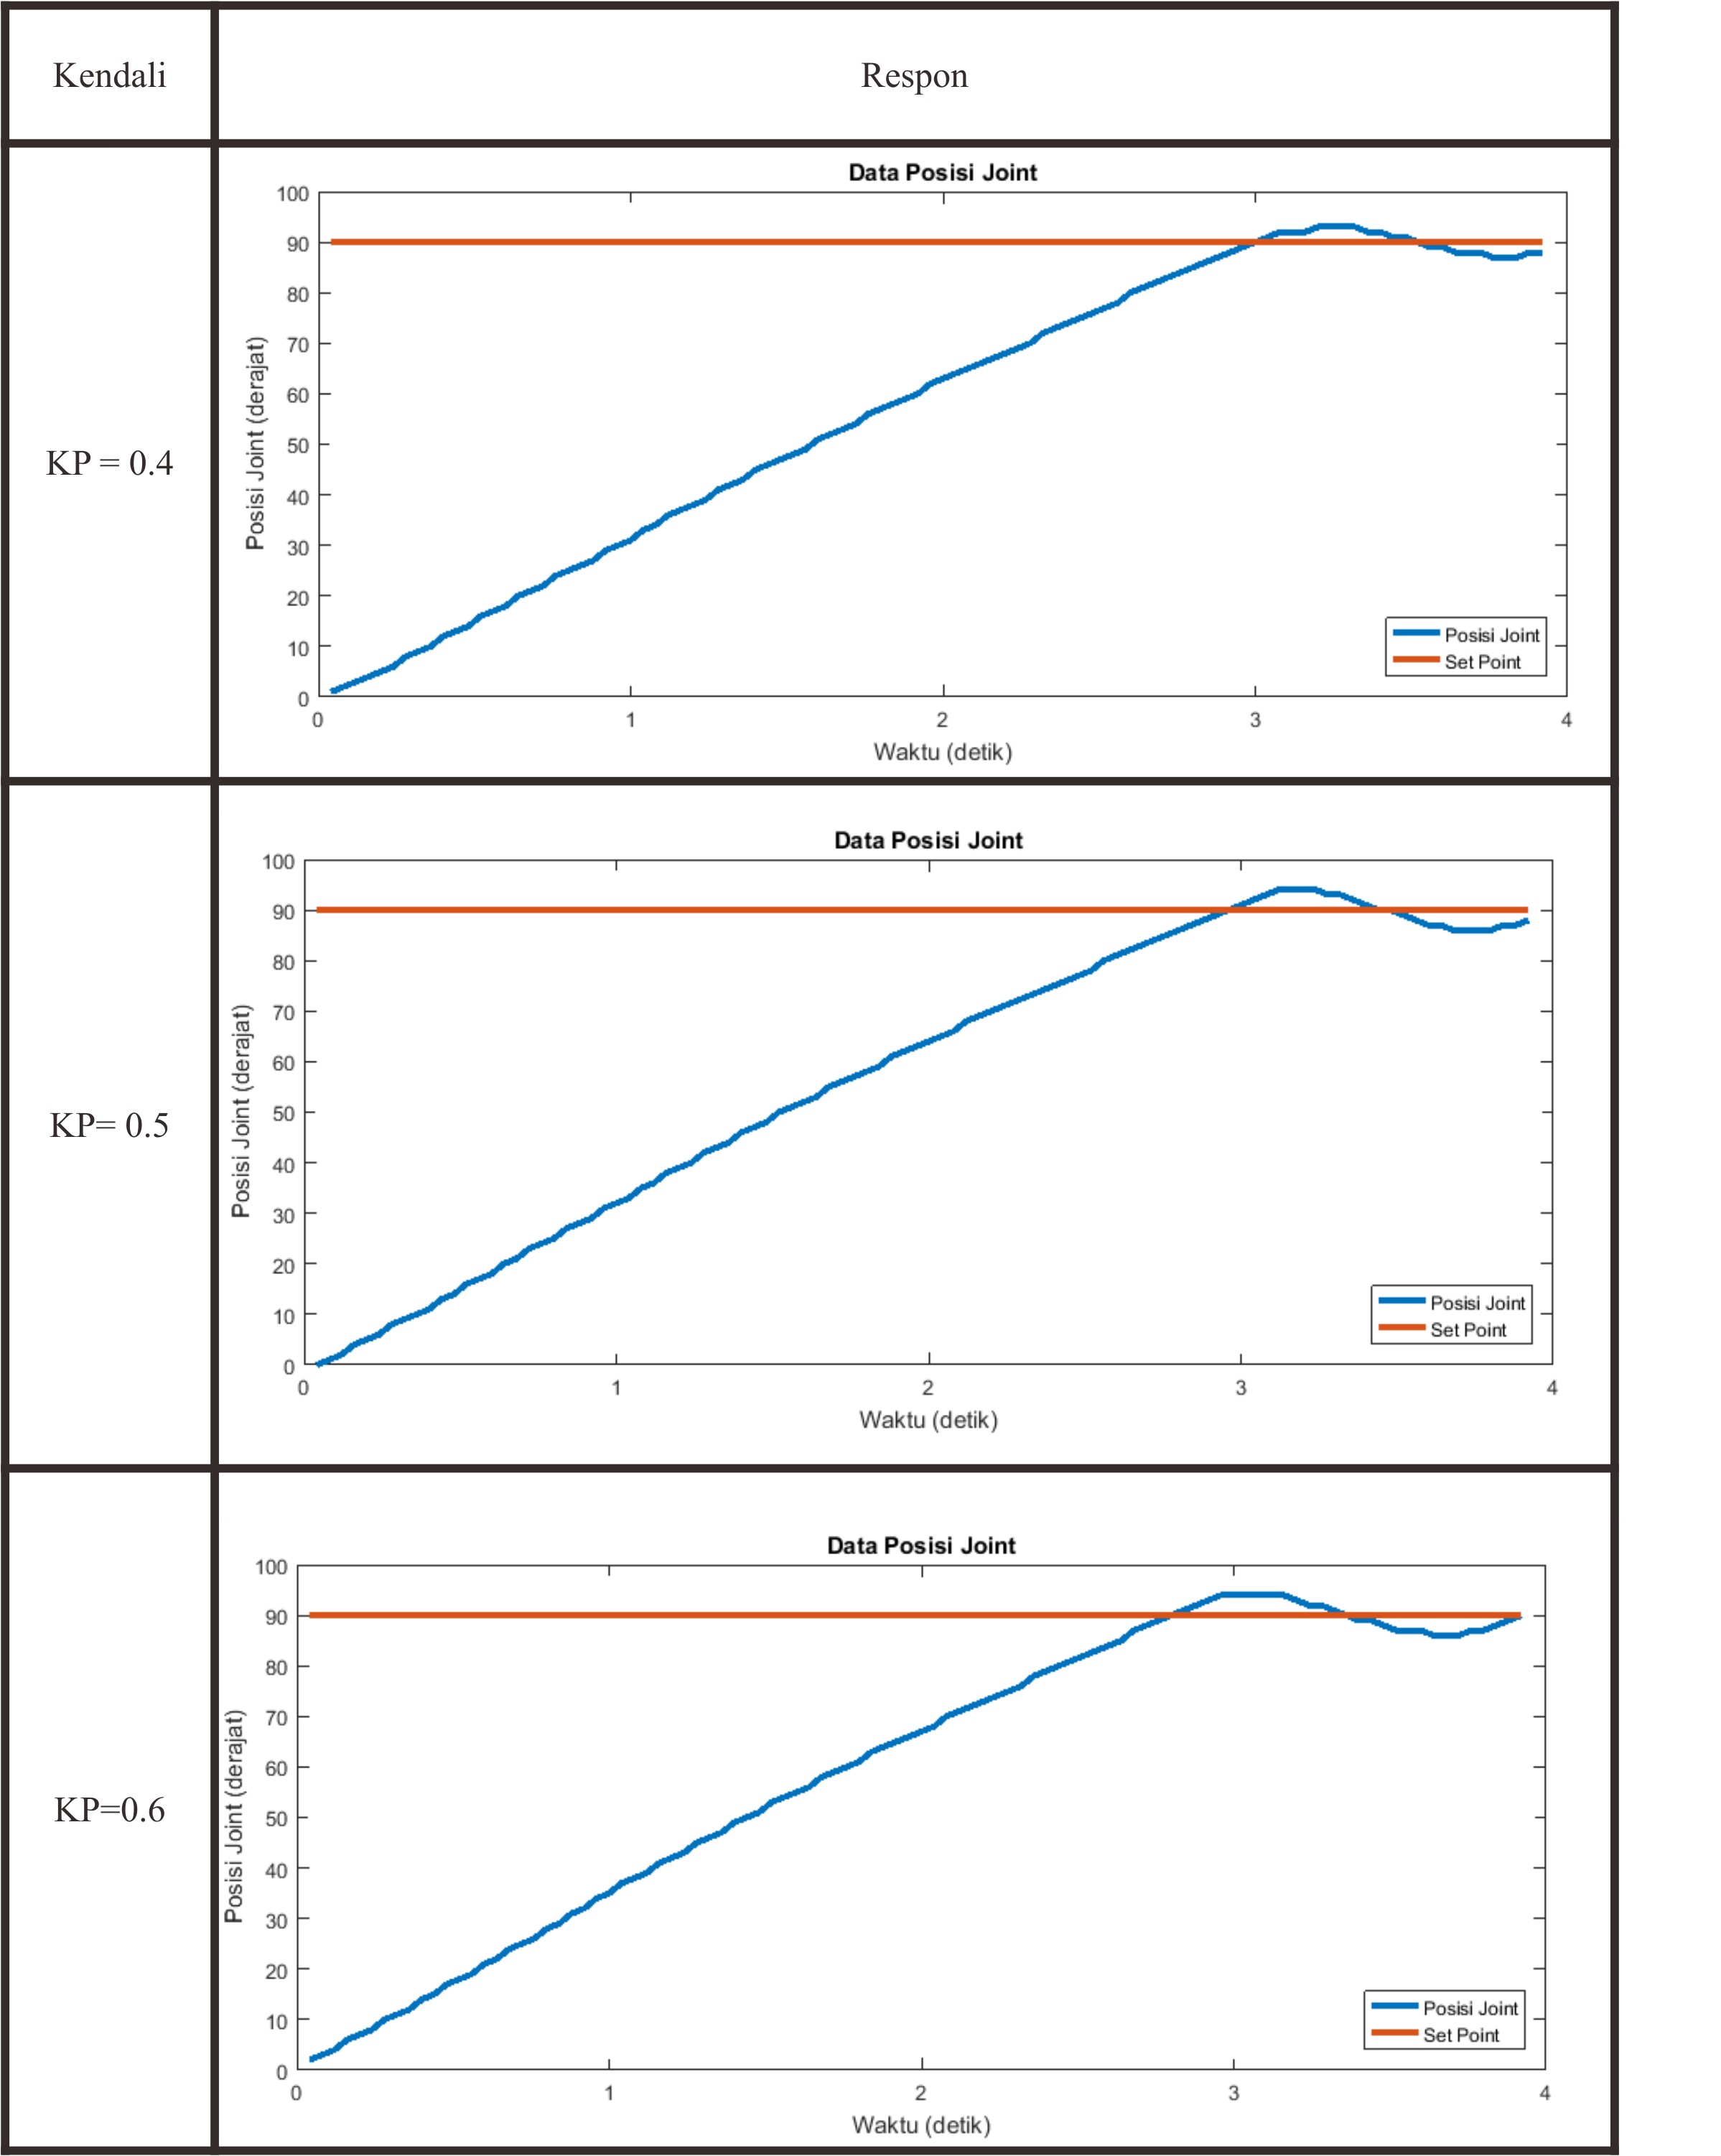
\includegraphics[width=13cm]{gambar/kendali2.png}
\end{figure}

\begin{figure}[H]
	\centering
	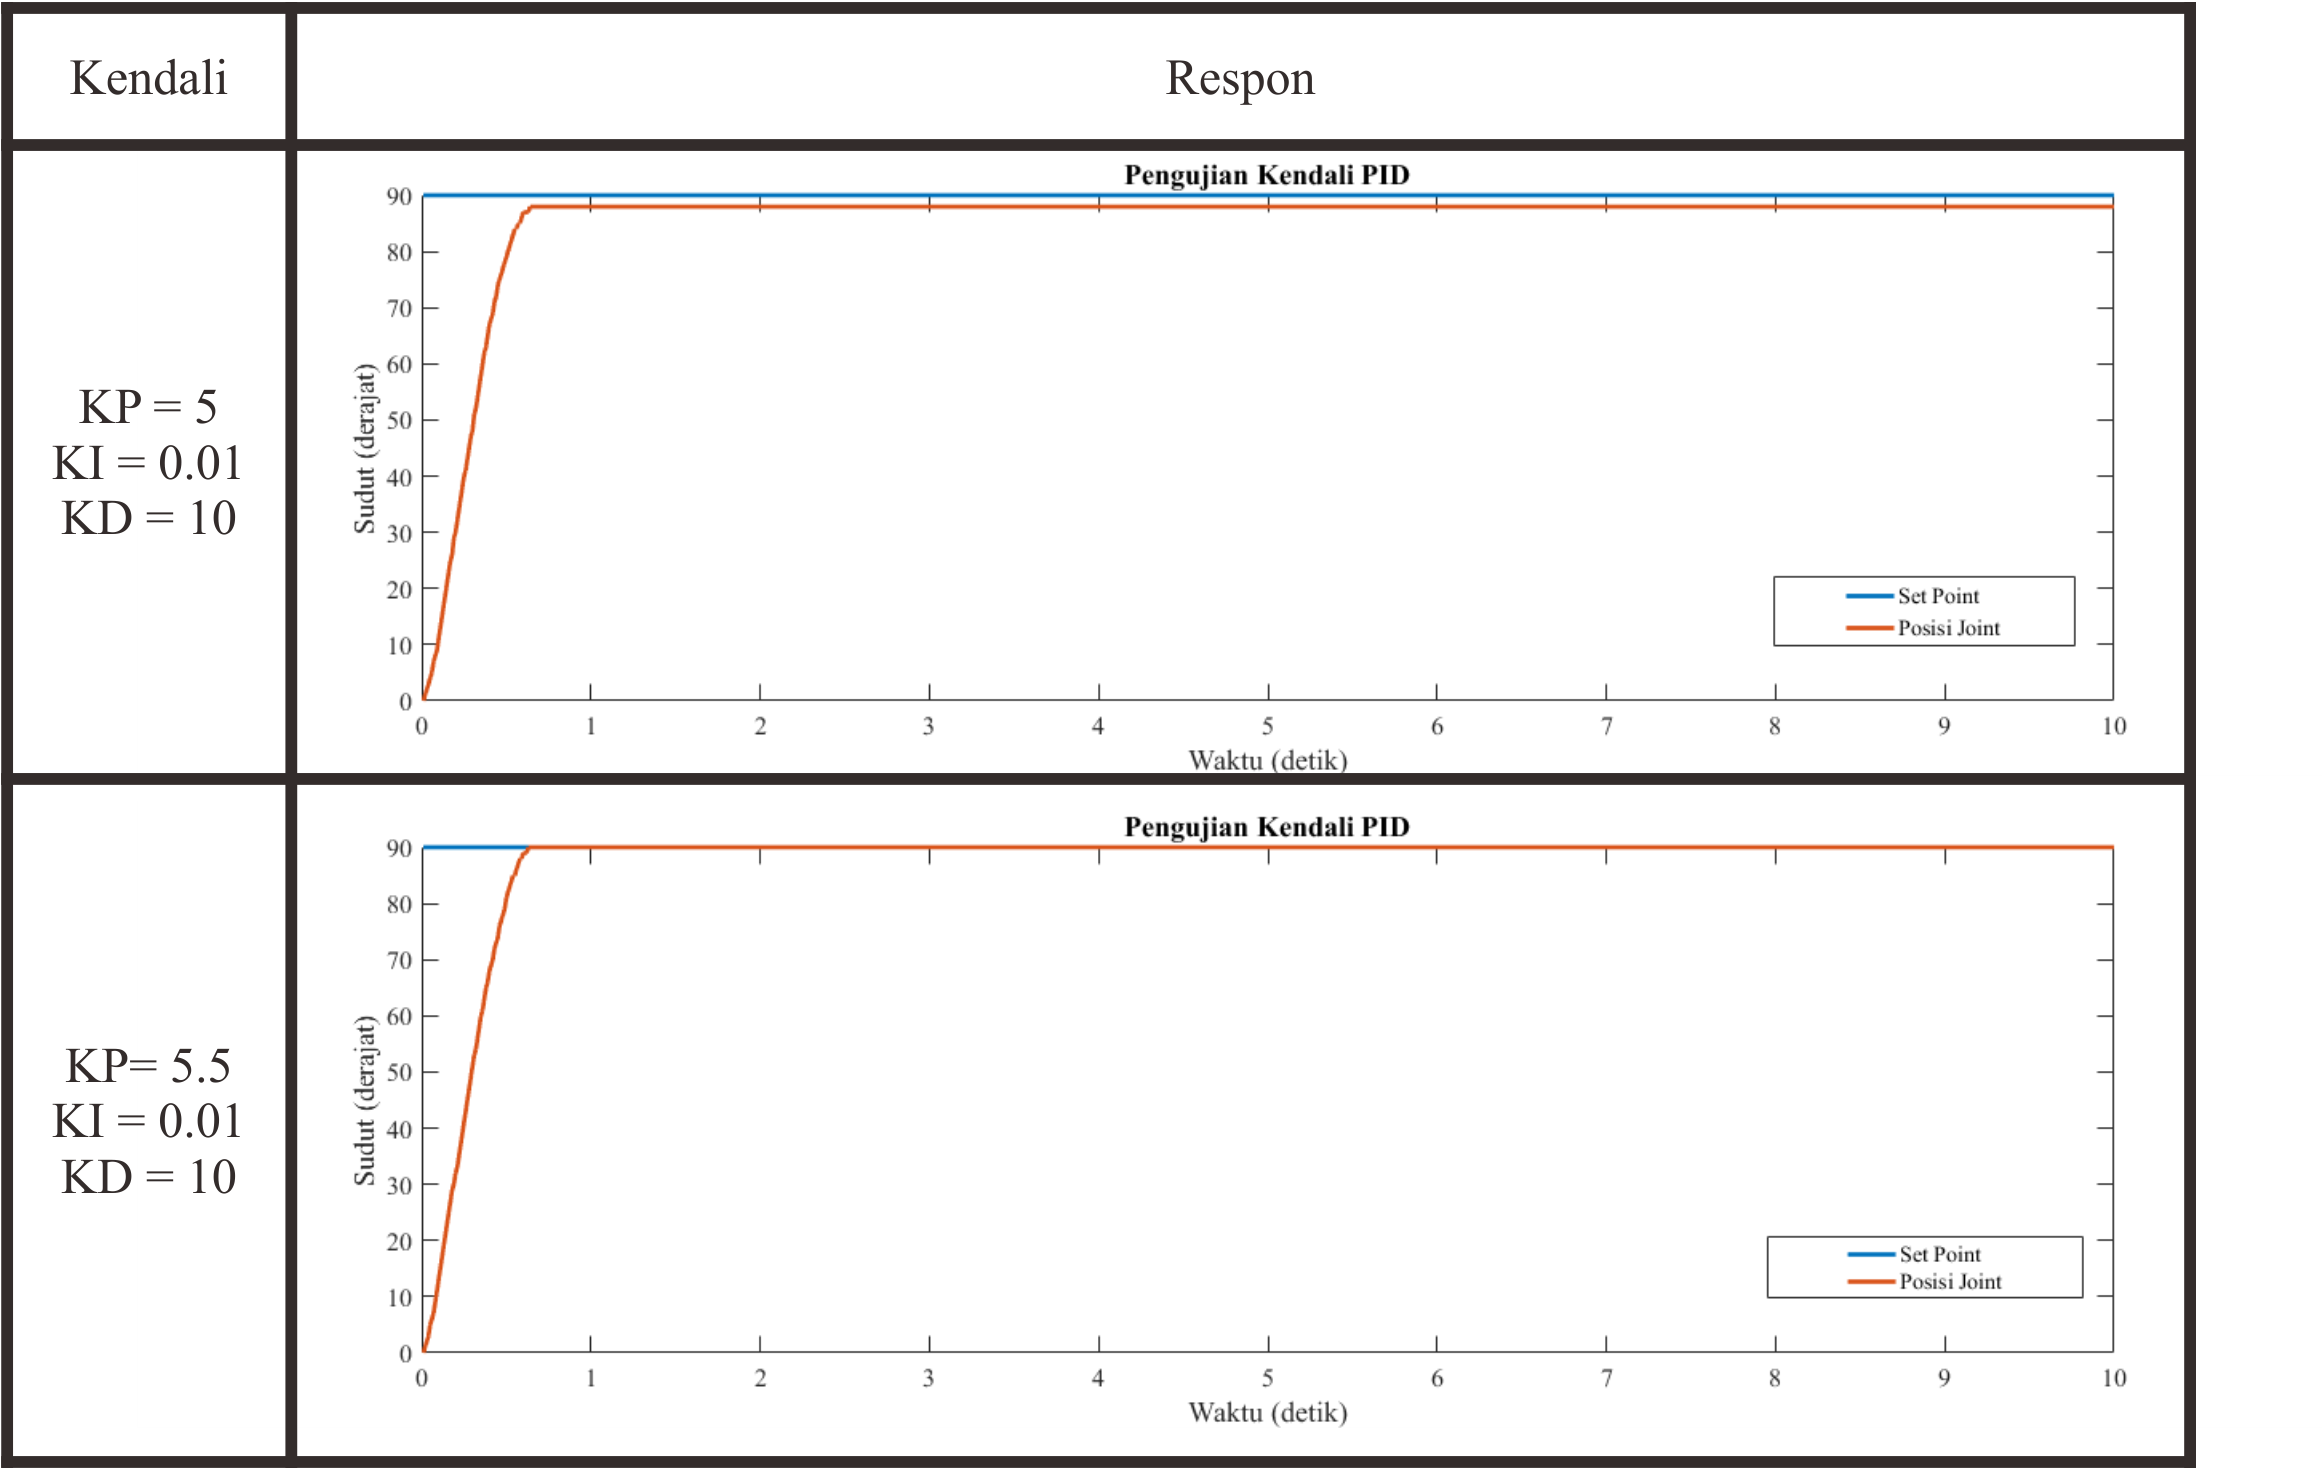
\includegraphics[width=13cm]{gambar/kendali3.png}
	\caption{Data Kendali Posisi}
	\label{pic.kendali}
\end{figure}

Dari beberapa nilai Kp yang coba diberikan kedalam robot lengan SCARA Serpent, terlihat bahwa respon yang didapat beraneka ragam. Respon terbaik adalah respon yang dapat mencapai posisi yang ditentukan dengan cepat dan nilai tersebut tetap stabil hingga pada nilai yang dimasukkan berbeda. Dari beberapa pengujian kendali proposional seperti yang ditunjukkan pada Gambar \ref{pic.kendali} terlihat bahwa respon dengan nilai Kp 0.2 merupakan respon terbaik. Hal ini berdasarkan dari besar nilai yang terukur sama dengan nilai yang dimasukkan dan tetap stabil atau tidak berubah-ubah dibandingkan dengan nilai Kp yang dimasukkan lainnya.
\section{Pengujian Simulasi Robot Lengan}
Pada pengujian ini, dilakukan serangkaian simulasi robot lengan untuk melakukan pergerakan sesuai dengan data yang diberikan melalui GUI yang telah dibuat. Simulasi ini menggunakan semua komponen yang ada di dalam perancangan, diantaranya robot SCARA Serpent, \textit{workspace}, catu daya, komputer personal, GUI Processing IDE, dan objek.

Pertama, robot SCARA Serpent berada posisi normal yang berarti pada posisi lurus searah dengan sumbu $y$. Robot SCARA Serpent akan mulai bergerak pada saat nilai data pada Processing IDE telah didapatkan dan kemudian dikirimkan ke Arduino Mega 2560. Proses pemilihan data pada Processing IDE dilalui pada sebuah GUI yang telah dibuat sesuai dengan fungsi dari robot SCARA Serpent. Pada GUI terdapat beberapa pilihan dalam memberikan sebuah nilai masukan. 

Kedua, robot SCARA Serpent akan mulai bergerak menuju posisi seperti data yang dimasukkan dan kemudian berhenti pada posisi tersebut dan mengambil objek yang dibawa oleh \textit{end-effector} pada posisi akhir.  Pergerakan \textit{end-effector} ditenagai oleh tekanan udara pada sebuah kompresor yang dikontrol oleh\textit{ valve pneumatic} yang diotaki oleh TIP31. Posisi akhir merupakan posisi dimana semua objek dikumpulkan. Setelah melakukan satu pekerjaan tersebut, robot SCARA Serpent kembali pada posisi normal dan menunggu data yang diberikan kembali oleh Processing IDE.  


